\documentclass[11pt,serif,mathserif,compress,hyperref={colorlinks}]{beamer}
\mode<presentation>
\usepackage{pgf}
\usepackage{pgfpages}
\usepackage[T1]{fontenc}
\usepackage[utf8]{inputenc}

\usepackage{lmodern}
\usepackage{lastpage}
\usepackage{comment}
\usepackage{geometry}
\usepackage[most]{tcolorbox}
\tcbuselibrary{skins}
\usepackage{beamerthemesplit}
\usepackage{amsmath, amsfonts, epsfig, xspace}
\usepackage{pstricks,pst-node}
\usepackage{multimedia}
\usepackage{pifont}   % zapf dingbats
\usepackage{marvosym} % MarVoSym dingbats
\usepackage{wasysym}
%\usepackage{animate}

\usepackage{graphicx}% for including figures
\usepackage{tikz}
\usepackage[tikz]{bclogo}
\usetikzlibrary{positioning,decorations.pathreplacing,arrows}
\usepackage{tikzsymbols}

\setlength{\parindent}{0pt}

%%%%%%%%%%%%%%%%%%  Couleurs %%%%%%%%%%%%%%%%%%%%%%%%%%%
\definecolor{mauve}{rgb}{0.5,0,0.7}
\definecolor{carmin}{rgb}{0.7,0,0}
\definecolor{bleu}{rgb}{0,0,0.7}
\definecolor{marron}{rgb}{0.6,0.35,0}
\definecolor{vert}{rgb}{0,0.5,0}
\definecolor{gris}{rgb}{0.9,0.9,0.9}
\definecolor{no}{rgb}{1,0.9,1}
%%%%%%%%%%%%%%%%%%%%%%%%%%%%%%%%%%%%%%%%%%%%%%%%%%%%%%%%%%

\definecolor{White}        {rgb}{1.0,1.0,1.0}

\definecolor{VeryDarkBlue} {RGB}{0,0,153}
\definecolor{DarkBlue}     {rgb}{0.0,0.0,0.6}
\definecolor{Blue}         {rgb}{0.0,0.0,1.0}
\definecolor{MidBlue}      {rgb}{0.6,0.6,1.0}
\definecolor{LightBlue}    {rgb}{0.8,0.8,1.0}
\definecolor{VeryLightBlue}{rgb}{0.9,0.9,1.0}

\definecolor{Gray}{rgb}{0.7,0.7,0.7}
\definecolor{LightGray}{rgb}{0.94,0.94,0.94}

\definecolor{DarkGreen}{rgb}{0,0.6,0}
\definecolor{MidGreen}{rgb}{0.6,1,0.6}
\definecolor{LightGreen}{rgb}{0.88,1,0.88}
\definecolor{VeryLightGreen}{rgb}{0.9,1,0.9}

\definecolor{Yellow}{rgb}{1,1,0.4}
\definecolor{MidYellow}{rgb}{1,1,0.5}
\definecolor{LightYellow}{rgb}{1,1,0.6}
\definecolor{VeryLightYellow}{rgb}{1,1,0.9}

\definecolor{DarkRed}{rgb}{0.7,0.,0.}
\definecolor{Red}{rgb}{0.8,0.,0.}
\definecolor{LightRed}{rgb}{1,0.8,0.8}
\definecolor{VeryLightRed}{rgb}{1,0.9,0.9}

\definecolor{Mauve}{rgb}{0.7,0.,0.7}

\definecolor{Magenta}{rgb}{1,0.,1}
\definecolor{LightMagenta}{rgb}{1,0.5,1}

\definecolor{Chocolate}{rgb}{0.54,0.2,.004}
\definecolor{DarkChocolate}{RGB}{103,38,.00}

\definecolor{DarkOrange}{rgb}{0.65,0.35,0.}
\definecolor{Orange}{rgb}{.9,0.4,0.}
\definecolor{LightOrange}{rgb}{1,0.8,0.5}

\definecolor{Brown}{rgb}{0.4,0.4,0.}

\definecolor{LightCyan}{rgb}{0.5,1.,1.}

\definecolor{PBG} {rgb}{1.0,1.0,0.6}
\definecolor{PTXT}{rgb}{0.2,0.2,0.0}
\definecolor{IBG} {rgb}{0.8,0.8,1.0}
\definecolor{ITXT}{rgb}{0.2,0.2,0.0}
\definecolor{OBG} {rgb}{0.8,1.0,0.8}
\definecolor{OTXT}{rgb}{0.0,0.4,0.0}

\newcommand{\CommentVeryLightBlue}[1]{{\textcolor{VeryLightBlue}{#1}}}
\newcommand{\CommentWhite}[1]{{\textcolor{White}{#1}}}

\newcommand{\VeryDarkBlue}[1]{\textcolor{DarkBlue}{#1}}
\newcommand{\DarkBlue}[1]{\textcolor{DarkBlue}{#1}}
\newcommand{\Blue}[1]{\textcolor{Blue}{#1}}
\newcommand{\LightBlue}[1]{\textcolor{LightBlue}{#1}}
\newcommand{\VeryLightBlue}[1]{\textcolor{VeryLightBlue}{#1}}

\newcommand{\DarkGreen}[1]{\textcolor{DarkGreen}{#1}}
\newcommand{\LightGreen}[1]{\textcolor{LightGreen}{#1}}
\newcommand{\VeryLightGreen}[1]{\textcolor{VeryLightGreen}{#1}}
\newcommand{\MidGreen}[1]{\textcolor{MidGreen}{#1}}

\newcommand{\DarkRed}[1]{\textcolor{DarkRed}{#1}}
\newcommand{\Red}[1]{\textcolor{red}{#1}}
\newcommand{\LightRed}[1]{\textcolor{LightRed}{#1}}
\newcommand{\VeryLightRed}[1]{\textcolor{VeryLightRed}{#1}}

\newcommand{\Gray}[1]{\textcolor{gray}{#1}}

\newcommand{\Black}[1]{\textcolor{black}{#1}}

\newcommand{\White}[1]{\textcolor{white}{#1}}

\newcommand{\Mauve}[1]{\textcolor{Mauve}{#1}}

\newcommand{\LightMagenta}[1]{\textcolor{LightMagenta}{#1}}
\newcommand{\Magenta}[1]{\textcolor{Magenta}{#1}}

\newcommand{\DarkOrange}[1]{\textcolor{DarkOrange}{#1}}
\newcommand{\Orange}[1]{\textcolor{Orange}{#1}}
\newcommand{\LightOrange}[1]{\textcolor{LightOrange}{#1}}

\newcommand{\DeepPurple}[1]{{\textcolor[rgb]{0.3,0.,0.6}{#1}}}

\newcommand{\Brown}[1]{{\textcolor{Brown}{#1}}}
\newcommand{\Chocolate}[1]{\textcolor{Chocolate}{#1}}
\newcommand{\DarkChocolate}[1]{\textcolor{DarkChocolate}{#1}}

\definecolor{DBluePy}{RGB}{ 28, 78, 99}
\definecolor{BluePy} {RGB}{ 60,110,131}
\definecolor{MBluePy}{RGB}{200,210,240}
\definecolor{LBluePy}{RGB}{220,230,240}
\definecolor{DOranPy}{RGB}{248,194,  3}
\definecolor{OranPy} {RGB}{255,220, 70}
\definecolor{GreenPy}{RGB}{237,255,204}

\newcommand{\bsh}{\textbackslash}
\newcommand{\bshbsh}{\textbackslash\textbackslash}
\newcommand{\chevrons}{\ttfamily>\hspace*{-0.25mm}>\hspace*{-0.25mm}>\hspace*{0.28mm}\xspace}
\newcommand{\M}[1]{\Mauve{#1}}
\newcommand{\DG}[1]{\DarkGreen{#1}}
\newcommand{\DR}[1]{\DarkRed{#1}}
\newcommand{\B}[1]{\Blue{#1}}
\newcommand{\BPy}[1]{\BluePy{#1}}
\newcommand{\VDB}[1]{\VeryDarkBlue{#1}}
\newcommand{\DO}[1]{\DarkOrange{#1}}
\newcommand{\Or}[1]{\Orange{#1}}
\newcommand{\Choco}[1]{\Chocolate{#1}}
\newcommand*{\truc}{\Gray{\textbullet}}

\newcommand{\bif}[1]{{\ttfamily \M{#1}}}	% Python built in function
\newcommand{\typ}[1]{{\ttfamily \M{#1}}}  % Python built in type
\newcommand{\key}[1]{{\ttfamily \Or{#1}}}
\newcommand{\str}[1]{{\ttfamily \DG{#1}}}
\newcommand{\com}[1]{{\ttfamily \DR{#1}}}
\newcommand{\out}[1]{{\ttfamily \B{#1}}}
\newcommand{\command}[1]{{\ttfamily \Choco{#1}}}
\newcommand{\code}[1]{{\ttfamily \Choco{#1}}}
\newcommand{\file}[1]{{\ttfamily \VDB{#1}}}

\newcommand{\bifBF}[1]{\textbf{\bif{#1}}}	% Python built in function
\newcommand{\typBF}[1]{\textbf{\typ{#1}}}  % Python built in type
\newcommand{\keyBF}[1]{\textbf{\key{#1}}}
\newcommand{\strBF}[1]{\textbf{\str{#1}}}
\newcommand{\comBF}[1]{\textbf{\com{#1}}}
\newcommand{\outBF}[1]{\textbf{\out{#1}}}
\newcommand{\commandBF}[1]{\textbf{\command{#1}}}
\newcommand{\codeBF}[1]{\textbf{\code{#1}}}
\newcommand{\fileBF}[1]{\textbf{\file{#1}}}

\newcommand{\bfchoco}[1]{\textbf{\Chocolate{#1}}}
\newcommand{\bfdarkchoco}[1]{\textbf{\DarkChocolate{#1}}}


%Beamer theme [\usetheme{jlcKeynote}]
\renewcommand\sfdefault{phv}
\renewcommand\familydefault{\sfdefault}
\usetheme{default}
\usepackage{color}
\useoutertheme{default}
\usepackage{texnansi}
\usepackage{marvosym}
\definecolor{bottomcolour}{rgb}{0.32,0.3,0.38}
\definecolor{middlecolour}{rgb}{0.08,0.08,0.16}
\setbeamerfont{title}{size=\Huge}
\setbeamercolor{structure}{fg=gray!50!white}
\setbeamertemplate{frametitle}[default]%[center]
%\setbeamercolor{normal text}{bg=black, fg=white}
\setbeamertemplate{items}[circle]
\setbeamerfont{frametitle}{size=\Large}
\setbeamertemplate{navigation symbols}{} %no nav symbols
% Beamer theme

\useoutertheme[subsection=false]{miniframes}
\setbeamercolor{background canvas}{bg=gray!50!white}
\setbeamercolor{structure}{bg=white, fg=gray}
\setbeamercolor{frametitle}{fg=DarkChocolate, bg=gray!50}
\setbeamertemplate{itemize item}{\small\gray{$\CIRCLE$}}
\setbeamertemplate{itemize subitem}{\tiny\gray{$\CIRCLE$}}
\settowidth{\leftmargini}{\usebeamertemplate{itemize item}}
\addtolength{\leftmargini}{\labelsep}

\setbeamercovered{transparent}

\hypersetup{linkcolor=Yellow}
\hypersetup{citecolor=DeepPink4}
\hypersetup{urlcolor=DarkBlue}
\hypersetup{anchorcolor=Magenta}

\medskip
\title[\hspace*{.8\linewidth}\insertframenumber/\inserttotalframenumber]
{\\\medskip\fontsize{17}{17}\selectfont{\textbf{Projet UCIA}}
}

\subtitle{\bigskip\fontsize{12}{12}\selectfont{COPIL du 6 janvier 2025\\\smallskip Partie technique}
}

\author[{\tiny JLC -- 2025/01/06}\hspace*{.8\linewidth}]
       {\fontsize{12}{12}\selectfont{Jean-Luc.Charles\,@\,mailo.com} %\\[2mm]
         %\includegraphics[height=1.5cm]{images/logo-couleur-rvb-en.png}
       }

\institute{}

\date{}

\titlegraphic{
  \href{https://creativecommons.org/licenses/by-sa/4.0/}
       {
\includegraphics[height=8mm]{images/CC-BY-SA.jpeg}}     
}

\logo{}

%\tcbset{enhanced, boxrule=0.2pt, sharp corners, drop lifted shadow=black,
%  colback=Chocolate!25!white,colframe=Chocolate!75!black, fonttitle=\Large}

\tcbset{enhanced, boxrule=0.2pt, sharp corners, drop lifted shadow=black,
    width=1.0\textwidth, left=5pt, left skip=-5pt,
    colback=Chocolate!25!white,colframe=Chocolate!75!black}

% fix the bug between hyperref & lastpge packages:
\makeatletter
  \def\Hy@PageAnchorSlidesPlain{}%
  \def\Hy@PageAnchorSlide{}%
\makeatother

\begin{document}

\renewcommand{\ttdefault}[0]{lmtt}
\newcommand{\boldtt}[1]{{\ttfamily\bfseries #1}}

%====== # 1 ==================================================
\frame[plain]{\titlepage}
%=============================================================

\setbeamercolor{structure}{fg=gray!50!white}

%====== # 2 ==================================================
\begin{frame}{}
  
  %\vspace*{-3mm}%
  \begin{bclogo}[noborder=true, couleur=gray!50, couleurBarre=Chocolate, logo=\bctrombone, marge=0, margeG=-0.5]
    {\ Partie technique}
    \medskip
    \begin{itemize}
    \item Concepts et outils de l'IA \smallskip
    \item Études menées \smallskip
    \item Mise en oeuvre avec la carte RPi4 \smallskip
    \item Démonstration... \smallskip
    \end{itemize}
  \end{bclogo}
  
\end{frame}
%=============================================================

\section{Concepts et outils de l'IA}

\subsection{The historical way...}

%====== # 3 ==================================================
\begin{frame}{IA : Aspects historiques... de 1950 à 2000}
  \hspace*{-8mm}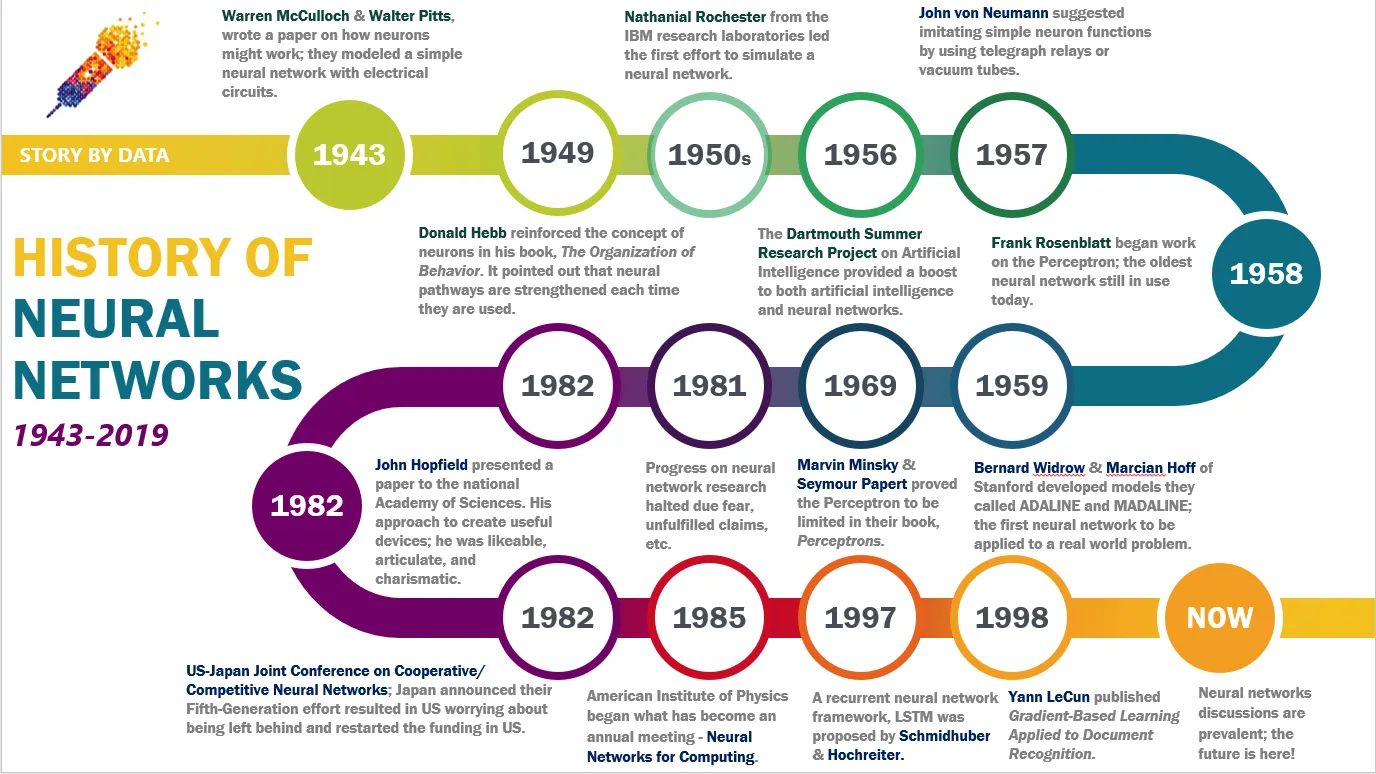
\includegraphics[width=1.13\textwidth]{images/Brief History of NN - Kate Strachnyi.png}\\
  \center{\footnotesize Source: \href{https://medium.com/analytics-vidhya/brief-history-of-neural-networks-44c2bf72eec}
    {Kate Strachni: "Brief History of Neural Netowrks", medium.com}}

\end{frame}
%=============================================================

%====== # 4 ==================================================
\begin{frame}{IA : Aspects historiques... l'accélération post 2012}
  \hspace*{-8mm}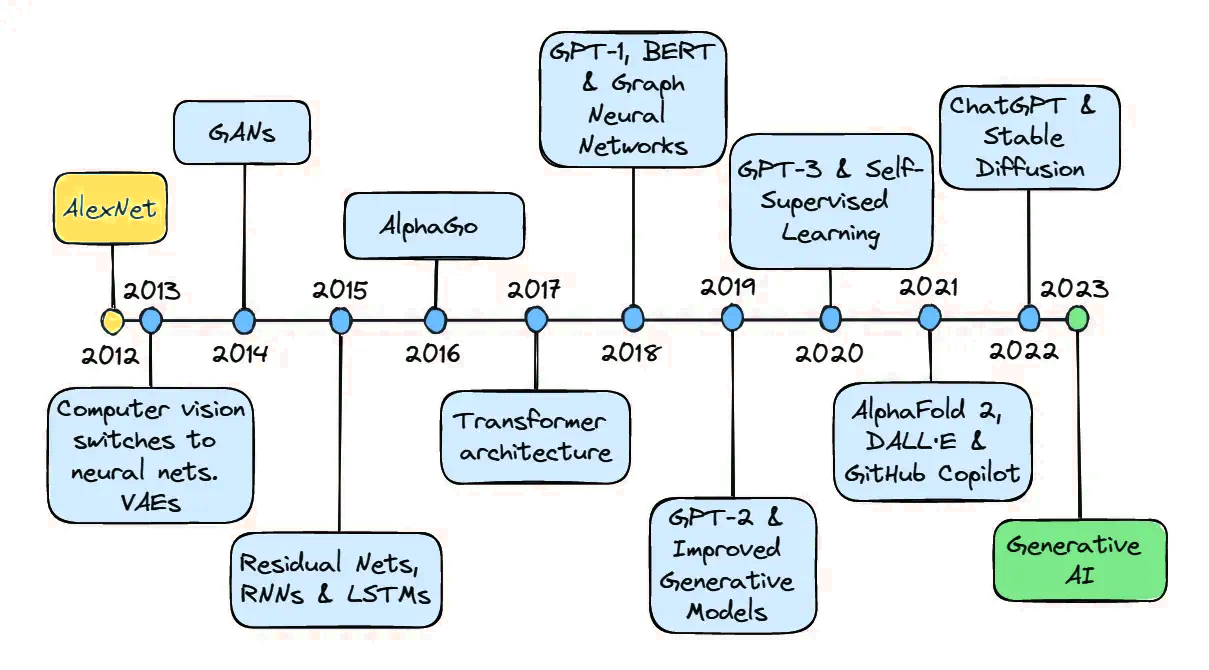
\includegraphics[width=1.1\textwidth]{images/Ten Years of AI in Review-2.png}\\
  \center{\footnotesize Source: \href{https://towardsdatascience.com/ten-years-of-ai-in-review-85decdb2a540}
    {Thomas A Dorfe: "Ten Years of AI in Review", medium.com}}
  
\end{frame}
%=============================================================

%====== # 5 ==================================================
\begin{frame}{IA : Aspects historiques post 2023 : accéleration}
    \hspace*{-12mm}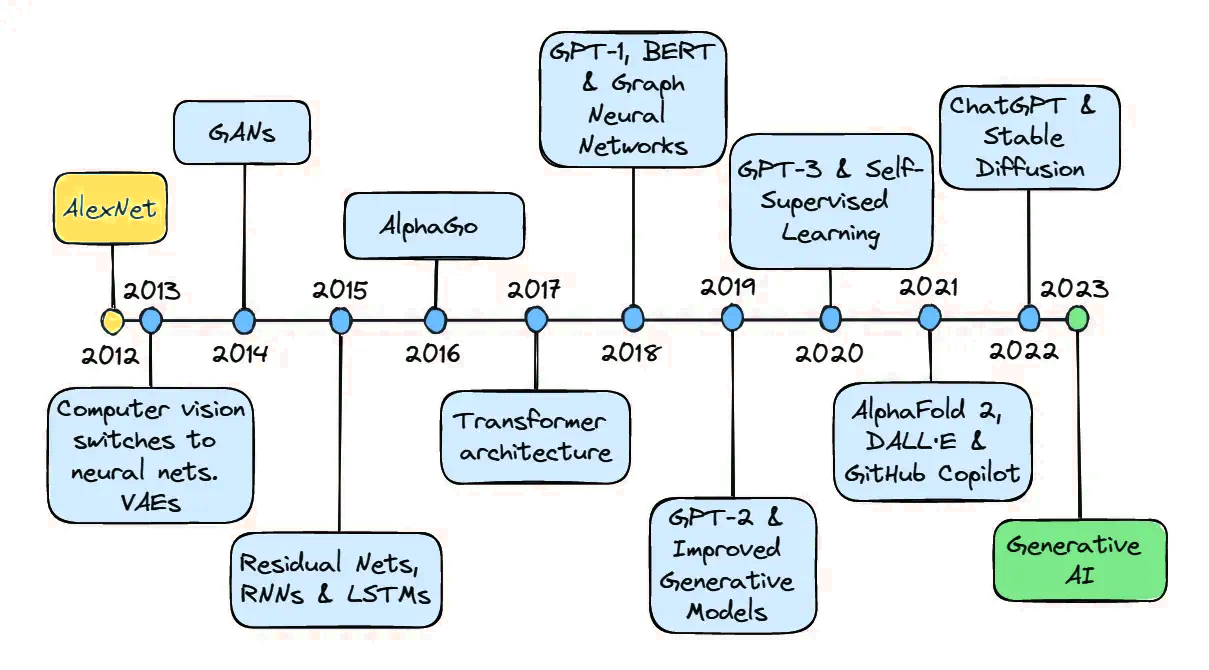
\includegraphics[width=.75\textwidth]{images/Ten Years of AI in Review-2.png}
    \begin{minipage}{\textwidth}
      \vspace*{-59.5mm}\hspace*{58mm}\frame{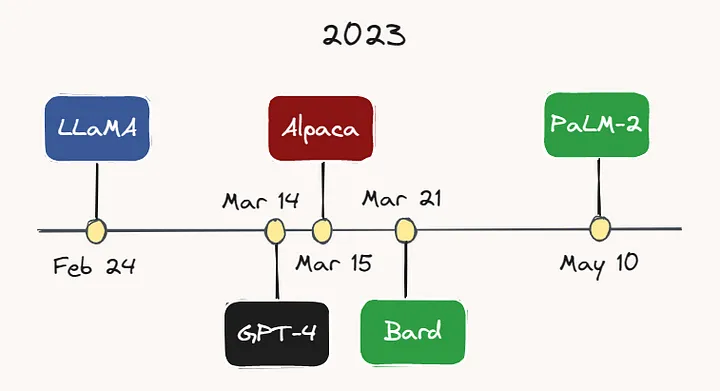
\includegraphics[width=0.51\textwidth]{images/post_2023-LLMs-Bots-2.png}}
    \end{minipage}\\
  \center{\footnotesize Source: \href{https://towardsdatascience.com/ten-years-of-ai-in-review-85decdb2a540}
    {Thomas A Dorfe: "Ten Years of AI in Review", medium.com}}
\end{frame}
%=============================================================

\subsection{Intelligence artificielle}

%====== # 6 ==================================================
\begin{frame}{Intelligence Artificielles ?}

  \vspace*{-2mm}
  \begin {bclogo}[noborder=true, couleur=gray!50, couleurBarre=Chocolate, logo=\bctrombone, margeG=-0.8]
    {}
    \vspace*{-5mm}
    Terme historiquement ''mal choisi'' %
    \footnote{{\tiny utilisé la première fois en 1956 par %
      \href{https://en.wikipedia.org/wiki/John\_McCarthy\_\%28computer\_scientist\%29}{John McCarthy},
      chercheur à Stanford, lors de la conférence de Dartmouth}}
    
    $\leadsto$ le sens actuel reste ambigu : de nombreuses définitions \\(contradictoires) existent selon les périodes et les auteurs...
    \end{bclogo}

  \visible<2->{

  \begin{itemize}
    {\small
    \item {\em '' ...the science of making computers do things that require intelligence when done by humans.}''
      {\tiny \href{http://www.alanturing.net/turing\_archive/pages/reference\%20articles/what\%20is\%20ai.html}{Alan Turing, 1940}}\smallskip
      
    \item {\em '' the field of study that gives computers the ability to learn without being explicitly programmed.''}
      {\tiny  \href{http://infolab.stanford.edu/pub/voy/museum/samuel.html}{Arthur Samuel, 1960}}\smallskip
      
    \item {\em '' A computer program is said to learn from experience E with respect to some class of tasks T and performance measure P,
      if its performance at tasks in T, as measured by P, improves with experience E.''}
      {\tiny \href{https://www.cs.cmu.edu/~tom/}{Tom Mitchell, 1997}}\smallskip
      
    \item Notion of {\em intelligent agent}, {\em rational agent} \\
      {\em ''...agent that acts in such a way as to reach the best solution or, in an uncertain environment, the best predictable solution.}''\\[-2mm]
      {\tiny  \href{http://aima.cs.berkeley.edu/translations.html}{Stuart Russel, Peter Norvig, ``Intelligence Artificielle'' 2015}}
    }
  \end{itemize}
  }
  
\end{frame}
%=============================================================

%====== # 7 ==================================================
\begin{frame}{Intelligences Artificielles ?}

  \textbf{Strong / General AI } (IA forte / générale)
  \only<2>{%
    \begin{itemize}
    \item Système IA qui {\bf pensent comme} les êtres humains, avec la capacité de raisonner en général.
    \item Tente aussi d'expliquer comment les êtres humains pensent.
    \item \Chocolate{nous n'en sommes pas encore là ?}
    \end{itemize}
  }
  
  \medskip
  \textbf{Weak / Narrow AI} (IA faible / spécialisée)
  \only<3>{% 
    \begin{itemize}
    \item Système IA qui semble {\bf se comporter comme} des être humains.
    \item Système IA conçu pour des tâches spécifiques.
    \item Ne renseigne pas sur la façon dont les êtres humains pensent.
    \item \Chocolate{Nous en sommes déjà là}... nous l'utilisons tous les jours !\\
      (anti-spam, reconnaissance voix/faciale, traduction...)
    \end{itemize}
  }

  \medskip
  \textbf{Multimodal AI} (IA multi-modale)
  \only<4>{%
    \begin{itemize}
    \item Système IA conçu pour traiter des entrées de nature multiple (texte, images, sons...).
    \end{itemize}
  }

  \only<5>{%
      \center\vspace*{-25mm}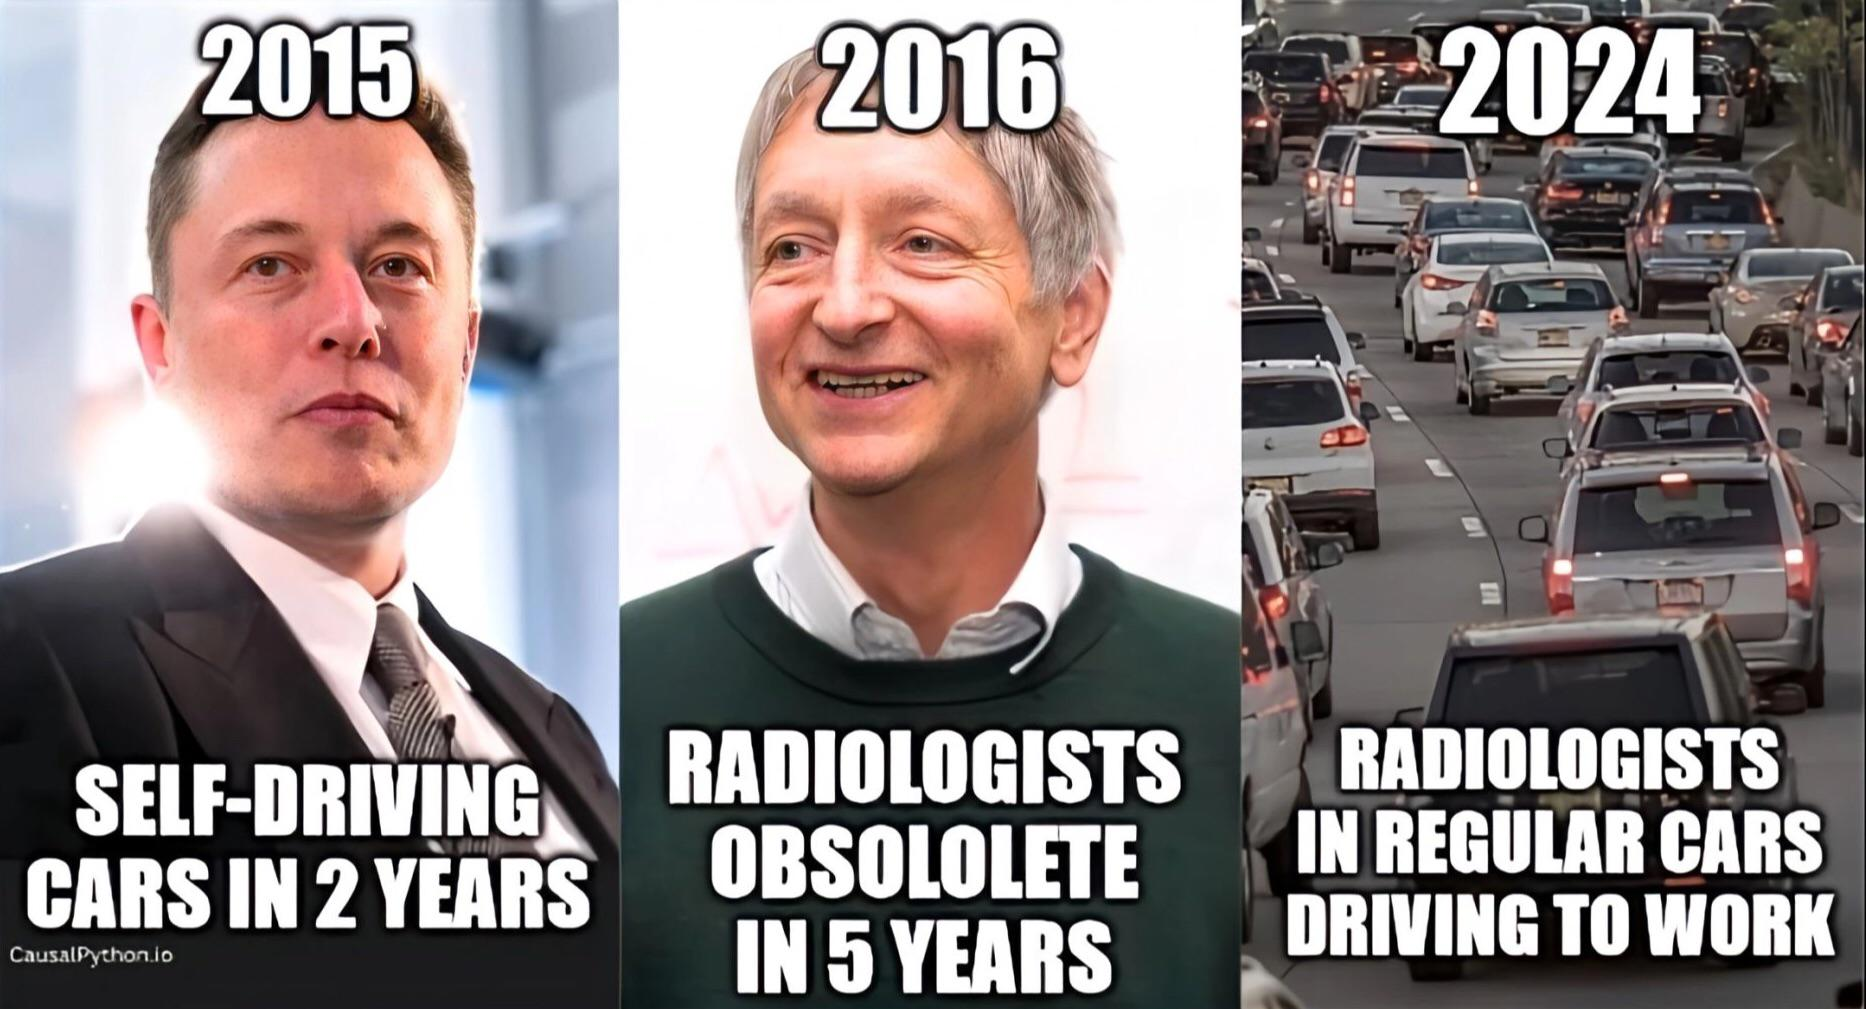
\includegraphics[height=63mm]{images/IA_predictions.jpeg}
  }
\end{frame}
%=============================================================

\subsection{Machine Learning}

%====== # 8 ==================================================
\begin{frame}{{\em Machine Learning}: un champ prometteur de l'IA}

  {\small Source \href{https://medium.com/machine-learning-for-humans/why-machine-learning-matters-6164faf1df12}
  {medium.com/machine-learning-for-humans/...}}\\[2mm]
  
  \hspace*{-10mm}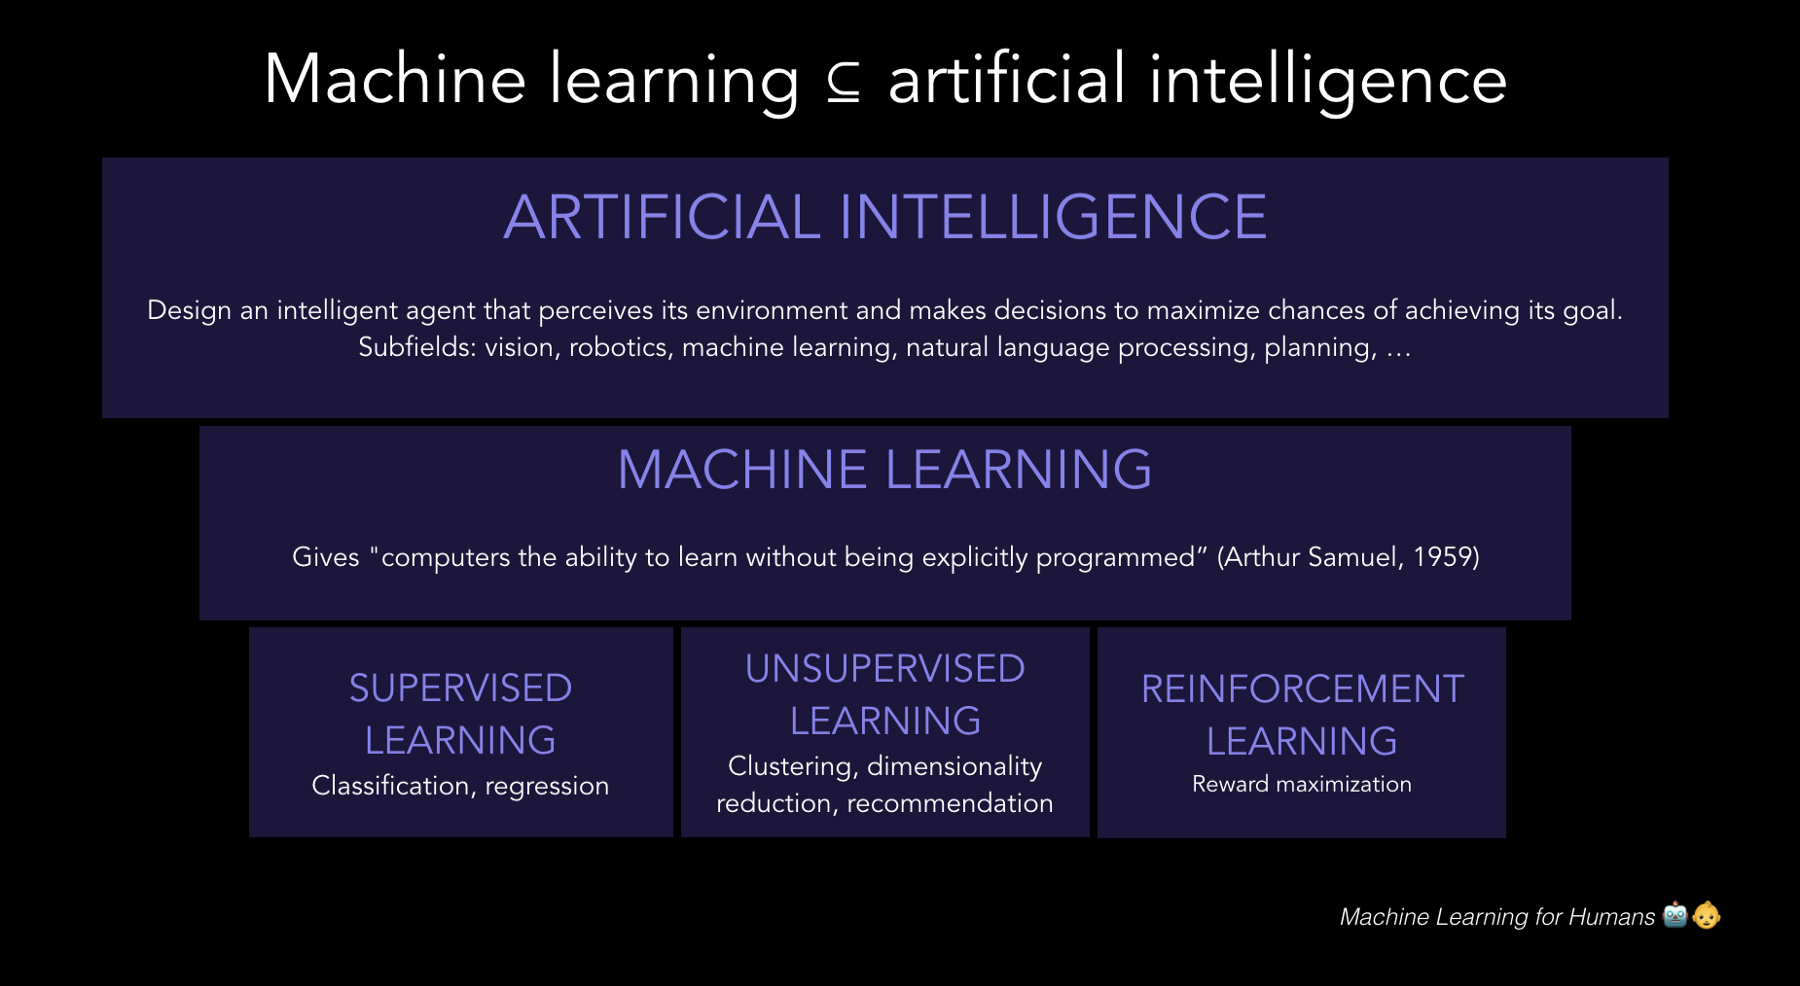
\includegraphics[width=1.2\textwidth]{images/AI-from_MachineLearningForHumans.png}
  \vspace*{-8mm}
  
\end{frame}
%=============================================================

%====== # 9 ==================================================
\begin{frame}{Branches du {\em Machine Learning}}

  %% Excellent: https://www.ibm.com/cloud/learn/machine-learning?lnk=fle

  \vspace*{-2mm}
  \begin{tcolorbox}[title={\bf Entraînement Supervisé} ({\em Supervised learning}), add to width=5mm, left skip=-6mm]
    Un jeu de  {\bf données labellisées} est utilisé pour l'entraînement :
    \begin{itemize}
    \item \textbf{Classification}
      \uncover<2->{
        \begin{itemize}
        \item Classification d'images
        \item Détection d'objets dans des images
        \item Reconnaissance de la parole...
        \end{itemize}
        }
    \item \textbf{Régression}
      \uncover<3->{
        \begin{itemize}
        \item Prévision de valeur...
        \end{itemize}
        }
    \item \textbf{Détection d'anomalie}
      %% anomaliy detection with supervised laerning suppose that there are no "new annomaly" in the
      %% datat set to process, because the anomalies have been learned and the algorithm will not
      %% recognize new anomaly that was not learned...
      \uncover<4->{
        \begin{itemize}
        \item Anti-spam
        \item Reconnaissance de défauts (appris)
        \item Prévision météo...
        \end{itemize}
        }
    \item $\cdots$
    \end{itemize}
  \end{tcolorbox}
  
\end{frame}
%=============================================================

%====== #10 ==================================================
\begin{frame}{Branches du {\em Machine Learning}}

  \vspace*{-2mm}
  \begin{tcolorbox}[title={\bf Entraînement non-supervisé} ({\em Unsupervised learning}), add to width=5mm, left skip=-6mm]
    Analyse et groupement de \textbf{données non-labellisées}:
    \begin{itemize}
    \item \textbf{Groupement}
      \uncover<2->{
        \begin{itemize}
        \item Exploration de données ({\em Data mining})
        \item Regroupement de données WEB
        \item Analyse de marché
        \item Analyse de données astronomiques...
        \end{itemize}
        }
    \item \textbf{Détection d'anomalie}
      \uncover<3->{
        \begin{itemize}
        \item Fabrication : détection de defauts (même nouveaux)
        \item Surveillance d'activité : fraude, défaillance, hacking
        \item Détection de {\em fake account} sur Internet...
        \end{itemize}
        }
    \item \textbf{Réduction de dimensionalité}
      \uncover<4->{
        \begin{itemize}
        \item Compression de données...
        \end{itemize}
        }
    \item $\cdots$
    \end{itemize}
  \end{tcolorbox}    
\end{frame}
%=============================================================

%====== #11 ==================================================
\begin{frame}{Branches du {\em Machine Learning}}

  \vspace*{-2mm}
  \begin{tcolorbox}[title={\bf Entraînement par renforcement} \\ Deep Reinforcement Learning (DRL), add to width=5mm, left skip=-6mm]
    Un {\em agent} apprend à piloter un {\em environment} en maximisant une \\{\em récompense} \textbf{reward} :
    \begin{itemize}

    \item \textbf{Contrôle des systèmes}
      \uncover<2->{
        \begin{itemize}
        \item Contrôle de robots, drones
        \item Optimisation de process de fabrication
        \item Négociation financière (boursière)...
        \end{itemize}
        }
    \item \textbf{Prise de décision}
      \uncover<3->{
        \begin{itemize}
        \item jeux vidéo
        \item Analyse financière...
        \end{itemize}
        }
    \item $\cdots$
    \end{itemize}
  \end{tcolorbox}

  \begin{minipage}{\textwidth}
    \vspace*{-24mm}\hspace*{42mm}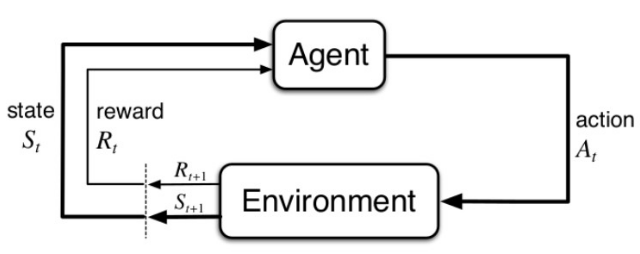
\includegraphics[width=.69\textwidth]{images/DRL.png}
  \end{minipage}

  \vfill
\end{frame}
%=============================================================

%====== #12 ==================================================
\begin{frame}{}

  %See \href{https://www.ibm.com/cloud/learn/machine-learning}{www.ibm.com/cloud/learn/machine-learning}
  
  \begin{tcolorbox}[title=Différents algorithmes du {\em Machine Learning}, add to width=7mm, left skip=-7mm]
    {\small
      \begin{minipage}[t]{.55\textwidth}
        \bfdarkchoco{Apprentissage Supervisé :}
        \begin{itemize}
        \item<1-> \only<1>{Réseau de neurones}\only<2->{\Blue{Réseau de neurones}}
        \item<1> Inférence Bayésienne
        \item<1> Random forest
        \item<1> Decision Tree
        \item<1> Support Vector Machine (SVM)
        \item<1> K-Nearest Neighbor
        \item<1> Régression Linéaire
        \item<1> Régression Logistique...
        \end{itemize}
      \end{minipage}\begin{minipage}[t]{.55\textwidth}
        \bfdarkchoco{Apprentissage non-supervisé :}
        \begin{itemize}
        \item<1-> \only<1>{Réseau de neurones}\only<2->{\Blue{Réseau de neurones}}
        \item<1> Principal Composant Analysis
        \item<1> Singular Value Decomposition
        \item<1> K-mean \& Prob. clustering...
        \end{itemize}
        \medskip
        \bfdarkchoco{DRL :}
        \begin{itemize}
        \item<1-> \only<1>{Réseau de neurones (Q-learning, Actor-Critic, DDPG, PPO...)}%
          \only<2->{\Blue{Réseau de neurones}\\[5mm]} 
        \item<1> Monte Carlo
        \item<1> SARSA...
        \end{itemize}
        
      \end{minipage}
    }
  \end{tcolorbox}    
  \visible<3>{\center{Grande variété de domaines $\leadsto$ succès\\des \Blue{Réseaux de Neurones} artificiels}}
\end{frame}
%=============================================================

\subsection{Neural Networks}

%====== #13 ==================================================
\begin{frame}{Applications du {\em Machine Learning}}

  \begin{tcolorbox}[title=Vision par ordinateur, add to width=7mm, left skip=-8mm, height=65mm]
    \begin{minipage}[t][][t]{.7\textwidth}
      \begin{itemize}
      \item<2-> Classification d'images
      \item<3-> Détection d'objects 
      \item<4-> Segmentation (sémantique)
      \item<5-> Génération d'images\\
        {\tiny \href{https://www.leptidigital.fr/productivite/meilleurs-generateurs-images-ia-30857/}{Les 23 meilleurs générateurs d’images par IA (Gratuits et Pros)}}
      \item<6-> Estimation de pose
      \item<7-> Transfer de style
      \item<8-> Reconnaisance optique de caracètres ({\small Optical Character Recognition: OCR})
      \item<8-> ...
      \end{itemize}
    \end{minipage}%
    \hspace*{-10mm}\begin{minipage}[t][][b]{.4\textwidth}
      \only<2>{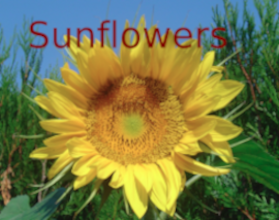
\includegraphics[width=1.\textwidth]{images/image_classification_sunflowers.png}}
      \only<3>{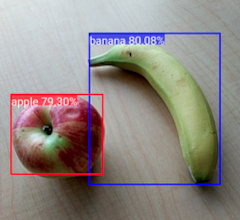
\includegraphics[width=1.\textwidth]{images/object_detection_aple-banana.png}\\
        {\centerline{\tiny source : \href{https://www.tensorflow.org/lite/examples/object_detection/overview}{Tensorflow}}}}
      \only<4>{\vspace*{18mm}\hspace*{-50mm}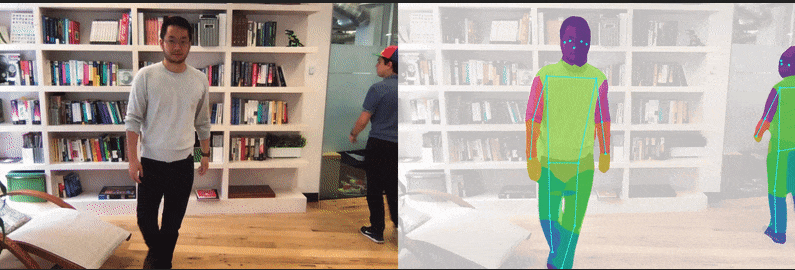
\includegraphics[width=2.\textwidth]{images/Semantic-segmentation.png}\\
        {\centerline{\tiny source : \href{https://blog.tensorflow.org/2019/11/updated-bodypix-2.html}{Tensorflow}}}}
      \only<5>{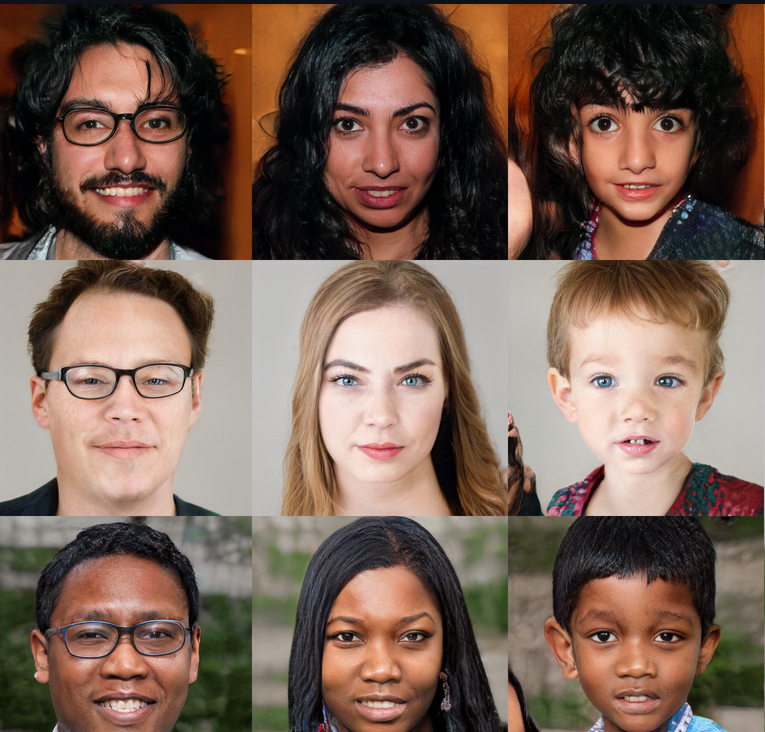
\includegraphics[width=1.\textwidth]{images/image_generation.png}\\
        {\centerline{\tiny source : \href{https://github.com/NVlabs/stylegan}{stylegan}}}}
      \only<6>{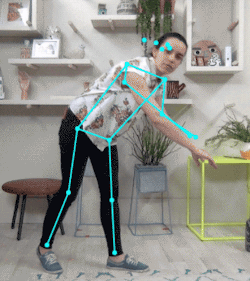
\includegraphics[width=.9\textwidth]{images/pose_estimation_TF.png}\\
        {\centerline{\tiny source : \href{https://blog.tensorflow.org/2021/05/next-generation-pose-detection-with-movenet-and-tensorflowjs.html}{Tensorflow}}}}
      \only<7>{\vspace*{-2mm}\hspace*{-60mm}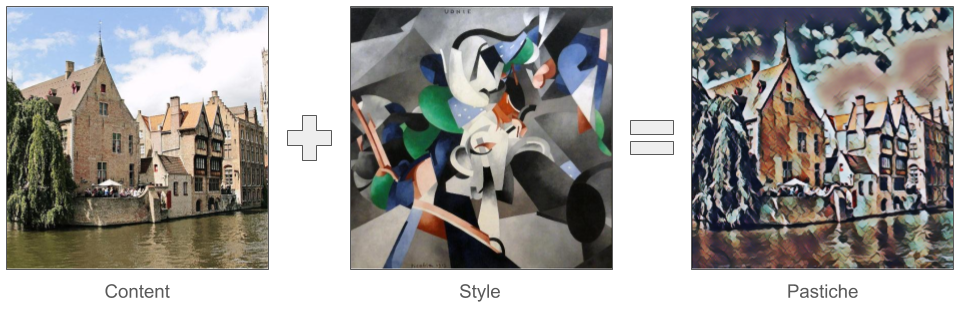
\includegraphics[width=2.3\textwidth]{images/style_transfer.png}\\
        {\centerline{\tiny source : \href{https://www.tensorflow.org/lite/examples/style_transfer/overview}{Tensorflow}}}}
      \only<8>{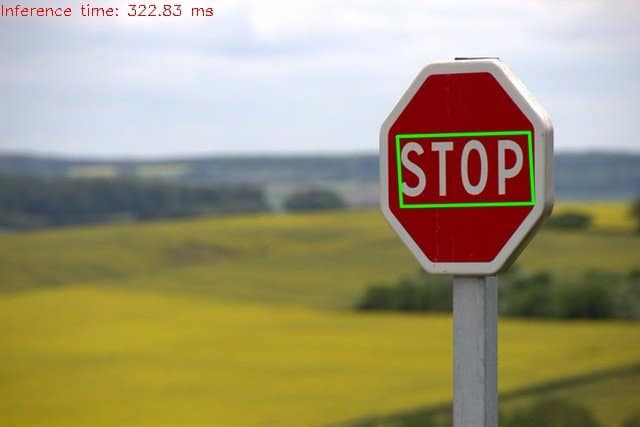
\includegraphics[width=1.\textwidth]{images/east-out-stop2.jpg}\\
        {\centerline{\tiny source : \href{https://www.tensorflow.org/lite/examples/optical_character_recognition/overview}{Tensorflow}}}}
    \end{minipage}
  \end{tcolorbox}
  
\end{frame}
%=============================================================

%====== #14 ==================================================
\begin{frame}{Applications du {\em Machine Learning}}

  \begin{tcolorbox}[title=Traitement du langage naturel ({\em{\small Natural Language Processing}}), add to width=7mm, left skip=-8mm]
    \begin{itemize}
    \item<2-> Natural Language Understanding (NLU) \smallskip
    \item<2-> Reconnaissance de la parole ({\em Speech recognition}) \smallskip
    \item<3-> Natural Language Generation (NLG) \smallskip
    \item<3-> Synthèse de la parole  ({\em Speech Synthesis, Text To Speech}) \smallskip
    \item<3-> Traduction de langues ({\em Machine Translation (languages)}) \smallskip
    \item<4-> Agent Conversationnel ({\em LLM ChatBots}) \smallskip
    \item<4-> ...
    \end{itemize}
  \end{tcolorbox}   
  
\end{frame}
%=============================================================

\subsection{Aspects infomatiques}

%====== #15 ==================================================
\begin{frame}{Aspects infomatiques}
  
  \tikzset{%
  neuron/.style={
    circle,
    draw,
    minimum size=1cm,
    font=\large
  },
  squa/.style={
    draw,
    inner sep=2pt,
    font=\large,
    join = by -latex
  },
  }
  \begin{tcolorbox}[title=Le modèle du neurone artificiel]  
    %\hspace*{-.7cm}
    \begin{tikzpicture}[x=1.3cm, y=.9cm]

      \node [label=above:\parbox{2cm}{\centering Entrées}] at (0, 1.5) (x1)  {$x_1$};
      \node [] at (0, 0.5) (x2) {$x_2$};
      \node [] at (0, -0) (vdots) {$\vdots$};
      \node [] at (0, -0.7) (xn) {$x_n$};
      \node [label=above:\parbox{2cm}{\centering Biais}] at (2, 2) (bias) {$b$};
      \node [label=above:\parbox{2cm}{\centering Sortie}] at (4, 0.15) (y) {$y = f(\sum_i{w_{i}\,x_i} - b)$};
      
      \node [neuron/.try] (output) at (2,0.15) {\large{$\displaystyle{\Sigma | f}$}};
      
      \draw [o-latex] (x1) -- (output);
      \draw [o-latex] (x2) -- (output);
      \draw [o-latex] (xn) -- (output);
      \draw [o-latex] (bias) -- (output);
      \draw [->] (output) -- (y);

      \node [] at (1,1) () {$w_1$} ;
      \node [] at (1,.5) () {$w_2$} ;
      \node [] at (1, -0.45) () {$w_n$} ;
    \end{tikzpicture}
  \end{tcolorbox}
  \smallskip
  \visible<1->{Le \bfdarkchoco{neurone artificiel}:
    \begin{itemize}
    \item <2-> reçoit les \textbf{entrées} $(x_{i})_{i=1..n}$ affectées des \textbf{poids} $(w_i)_{i=1..n}$
    \item <3-> calcule la \textbf{somme pondérée} de ses entrées : $\sum_i{w_{i}\,x_i - b}$
    \item <4-> donne en \textbf{sortie} son activation : $f(\sum_i{w_{i}\,x_i} - b)$ \\calculée avec sa \textbf{activation function} $f$.
    \end{itemize}
  }

\end{frame}
%=============================================================

%====== #16 ==================================================
\begin{frame}{Aspects informatiques}
  
  \begin{tcolorbox}[add to width=.7cm, title={Exemples de fonctions d'activation courantes}]
    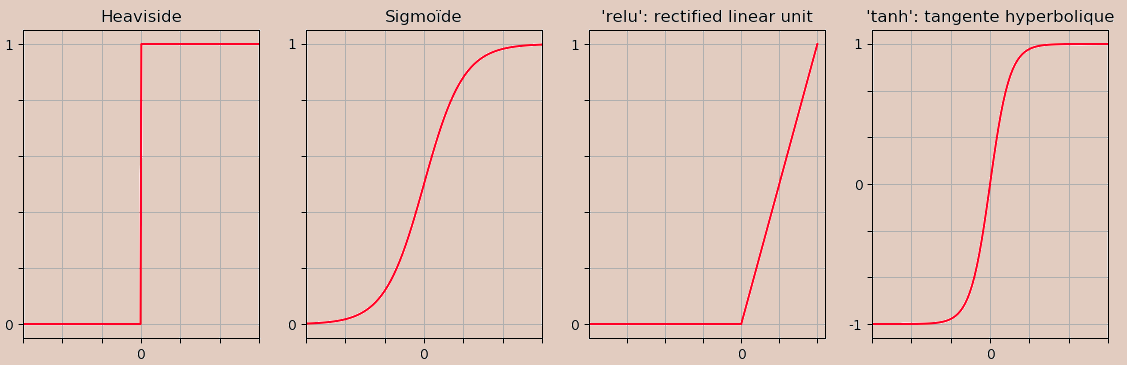
\includegraphics[width=1.\textwidth]{images/activ_functions-2.png}
  \end{tcolorbox}
  
  \visible<1->{La \bfdarkchoco{fonction d'activation}:
    \begin{itemize}
    \item <2-> Introduit un \textbf{comportement non-linéaire}, indispensable pour la réussite de l'apprentissage.
    \item <3-> Fixe la plage de sortie du neurone : $[-1, 1]$, $[0, 1]$, $[0, \infty[$...
    \end{itemize}
    }
  
\end{frame}
%=============================================================

%====== #17 ==================================================
\begin{frame}{Aspects informatiques}
  
  \begin{tcolorbox}[add to width=.7cm, title={Réseau de neurones artificiels}]

    Les neurones sont regroupés en couches pour former un \textbf{Réseaux de Neurones} artificiels (RN) 
    
    \smallskip
    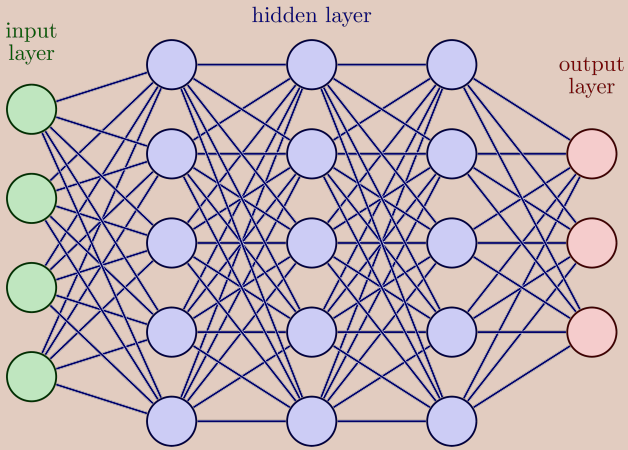
\includegraphics[width=.4\textwidth]{images/neural_networks-005-a.png}\hfill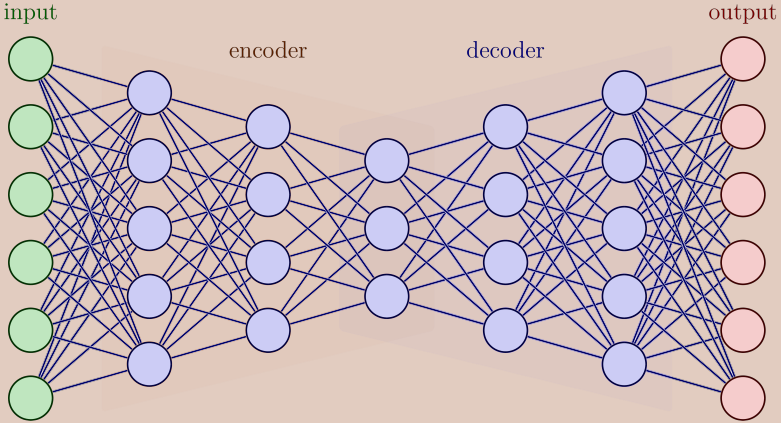
\includegraphics[width=.5\textwidth]{images/neural_networks-008-a.png}

  \end{tcolorbox}
  
\end{frame}
%=============================================================

%====== #18 ==================================================
\begin{frame}{Architecture des Réseaux de Neurones}

   \begin{tcolorbox}[title=Architectures dédiées à des applications spécifiques, add to width=7mm, left skip=-8mm, height=65mm]
     \begin{itemize}
     \item<2-> {\em \bfdarkchoco{Dense Neural Network}}%
       \only<2>{\\ La plus simple des architectures faite de couches successives de neurones, utilisant les algorithmes {\em Feed Forward} et {\em Back Propagation}}
     \item<3-> {\em \bfdarkchoco{Convolutional} (CNN)}%
       \only<3>{ - Réseau de Neurones Convolutionnel\\Principalement utilisé pour la classification d'images.}
     \item<4-> {\em \bfdarkchoco{Recurrent} (RNN)}%
       \only<4>{ - Réseau de Neurones Récurent\\Traitement des {\bf séries temporelles} (Exemple: {\em Long Short-Term Memory (LSTM)}).}
     \item<5-> {\em \bfdarkchoco{Auto Encoder} (AEN)}%
       \only<5>{-  Réseau de Neurones Auto-encodeur\\Réduction de dimentionnalité, compression, débruitage, détection d'anomalie...}
     \item<6-> {\em \bfdarkchoco{Generative Adversarial} (GAN)}%
       \only<6>{\\ génération de texte, images, musique...}
     \item<7-> {\em \bfdarkchoco{Transformers}}%
       \only<7>{\\ (2017) Traitement du langage naturel, puis aussi pour la classification d'images.}
     \item<8-> {\em \bfdarkchoco{Large Language Model} (LLM)}%
       \only<8>{\\ lecture de texte, sons, images... génération de texte, livres, images, parole, musique (Exemple: {\em ChatGPT, LLama}...)}
     \end{itemize}
   \end{tcolorbox}
   \uncover<9>{
     \center\footnotesize[Graphique synthétique animé :
       \href{https://chart-studio.plotly.com/~SolClover/90.embed?autosize=true&referrer=https\%3A\%2F\%2Ftowardsdatascience.com\%2F}{Saul Dobilas sur Medium}] }
\end{frame}
%=============================================================

\subsection{Societal issues}

%====== #19 ==================================================
\begin{frame}{Enjeux sociétaux de l'IA : {\bf Explicabilité}}

  devenue rapidement une priorité dans la recherche : \\
  $\leadsto$ {\bf xAI} : {\em {\bf Explicable} Artificial Intelligence} \\
  $\leadsto$ {\bf iML} : {\em {\bf Interpretable} Machine learning} \smallskip

  \begin{tcolorbox}[title={\bf Explicabilité} des Réseaux de Neurones (RN)]
    \begin{itemize}
    \item {\bf Inexplicabilité} des résultats calculés par les RN $\leadsto$ obstacle à leur diffusion.
    \item L'apprentissage profond avec les RN souvent dénigré comme une ''boîte noire'' par les scientifiques ayant une ''approche cartésienne''...
    \item La complexité grandissante des RN (LLM par exemple) rend l'explication simple de leurs décisions extrêmement difficile.
    \end{itemize}
  \end{tcolorbox}   
    
\end{frame}
%=============================================================

%====== #20 ==================================================
\begin{frame}{Enjeux sociétaux de l'IA : {\bf Prise de décision}}
  
  \begin{tcolorbox}[title={\bf Prise de décision}]
    \begin{itemize}
    \item Un nombre croissant de décisions dans des domaines sensibles (justice pénale, santé, assurance, défense...)
      confiées aux algorithmes ML source d'inquiétude...
    \item Les algorithmes de prise de décision reposent inévitablement sur des hypothèses
      (qualité des données d'apprentissage par exemple) souvent difficile à vérifier.
    \item Se pose la question de la transparence des algorithmes, des données d'entraînement ({\em Open Source} ).
    \end{itemize}
  \end{tcolorbox}   
    
\end{frame}
%=============================================================

%====== #21 ==================================================
\begin{frame}{Enjeux sociétaux de l'IA : {\bf Certification}}
  
  \begin{tcolorbox}[title={\bf Certification}]
    \begin{itemize}
    \item {\bf Évaluation} et {\bf Certification} des systèmes IA\\
      $\leadsto$ enjeu majeur pour leur intégration dans l'industrie. \medskip
    \item {\bf Certification} formelle des algorithmes de ML\\
      $\leadsto$ reste aujourd'hui un sujet de recherche :
      \begin{itemize}
      \item \href{https://www.lne.fr/fr/service/certification/certification-processus-ia}{LNE : Certification des processus pour l'IA}
      \item \href{https://www.hhi.fraunhofer.de/en/departments/ai/technologies-and-solutions/auditing-and-certification-of-ai-systems.html}
           {Fraunhoher : Audit et certification des systèmes d'IA}
      \end{itemize}
    \end{itemize}
  \end{tcolorbox}
    
\end{frame}
%=============================================================

\section{Étude}

%====== #22 ==================================================
\begin{frame}{}

  \vfill
  \center{\Large Études : entraînement d'un réseau de neurones \\[2mm] YOLO pour la détection de petits objets 3D\\[5mm]
    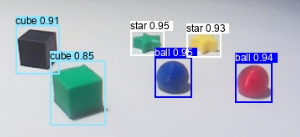
\includegraphics[width=.5\textwidth]{images/DetectionObjets.png}}
  \vfill
  Livrables: projet GiHb \href{https://github.com/cjlux/UCIA_ObjectDetection/tree/master}{UCIA\_ObjectDetection}
  \vfill

\end{frame}
%=============================================================

%====== #23 ==================================================
\begin{frame}{Détection d'objets 3D}
  
  Deux études menées en novembre-décembre 2024:
  
  \begin{tcolorbox}[title={Étude préliminaire (v1)}, add to width=.7cm, height=65mm]

    Objectifs :
    \begin{itemize}
    \item<1-> Faisabilité d'entraîner un réseau YOLO à détecter les petits objets 3D du projet UCIA
    \item<2-> Tester l'exploitation sur RPi4 d'un réseau YOLO entraîné.
    \end{itemize}
    \medskip
    \only<3->{
      Configuration :
      \begin{itemize}
      \item Caméra Raspberry standard montée sur trépied
      \item Entraînement des réseaux sur PC + carte graphique Nvidia
      \item Exploitation sur RPi4 4Go RAM des réseaux entraînés.
      \end{itemize}
      }
    \only<4>{\vspace*{-8.2cm}\center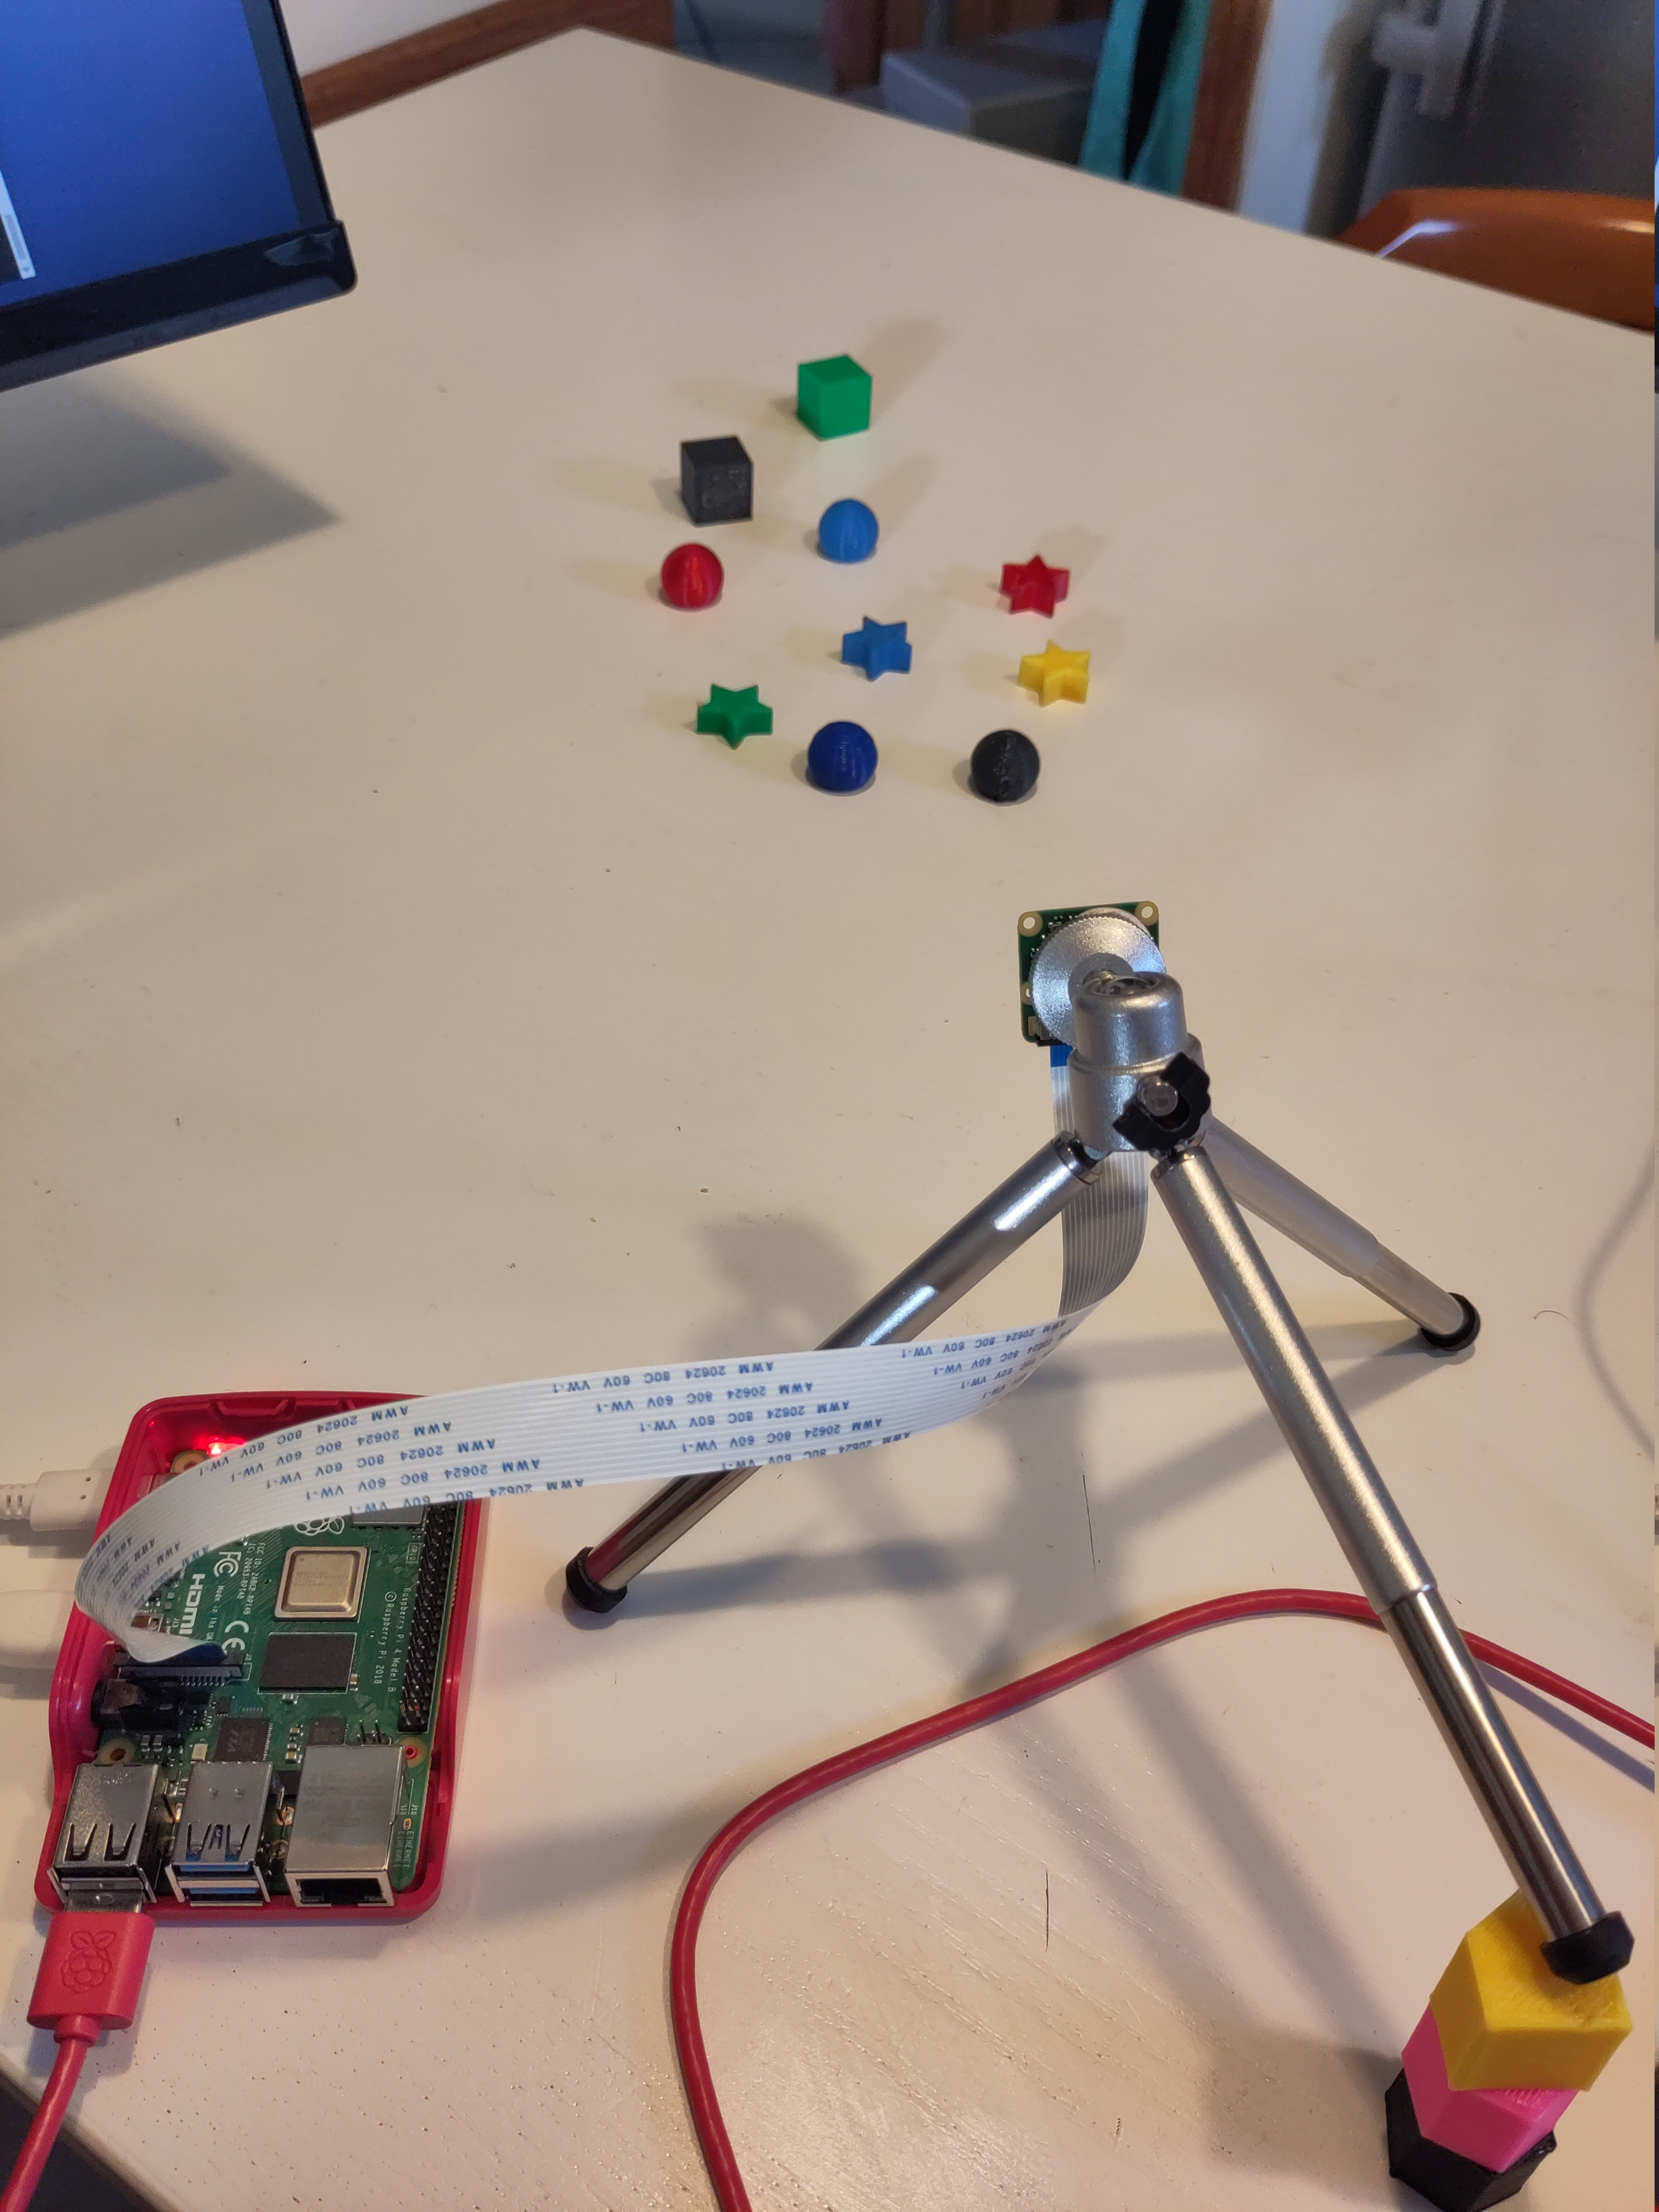
\includegraphics[width=.58\textwidth]{images/RPi4_Camera_V2 - 2.jpg}}
  \end{tcolorbox}
    
\end{frame}
%=============================================================

%====== #24 ==================================================
\begin{frame}{Détection d'objets 3D}
  
  \begin{tcolorbox}[title={Étude consolidée (v2)}, add to width=.7cm, height=70mm]
    Objectifs :
    \begin{itemize}
    \item<1-> Consolidation de l'entraînement de réseaux YOLO dans les conditions matérielles du CDC du projet UCIA
    \item<2-> Visualisation à distance (navigateur WEB, bureau à distance)
    \item<3-> Prototypage Python du déplacement du Thymio.
    \end{itemize}
    \medskip
    \only<4->{
      Configuration :
      \begin{itemize}
      \item Caméra Raspberry grand angle, fixée sur le support Thymio.
      \item Entraînement des réseaux sur PC + carte graphique Nvidia
      \item Exploitation sur RPi4 4Go RAM fixée sur le support Thymio.
      \end{itemize}
      }
    \only<5>{\vspace*{-5.2cm}\center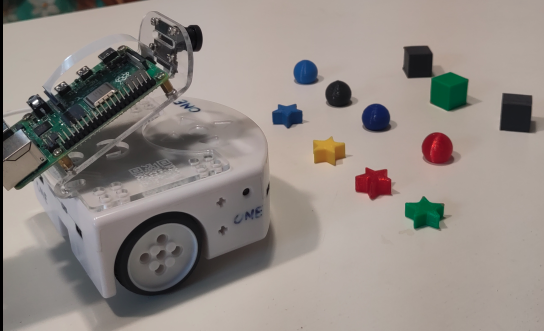
\includegraphics[width=.7\textwidth]{images/V2-Camera-Thymio.png}}
  \end{tcolorbox}
    
\end{frame}
%=============================================================

%====== #25 ==================================================
\begin{frame}{Détection d'objets 3D : Banque d'images annotées}
  
  \begin{tcolorbox}[title=Images de l'étude préliminaire (caméra Standard)]
    {\small Caméra Rasberry Standard, 62 images, 10 objets/images\\
      $\leadsto$ ~620 objets}
    
     \medskip\includegraphics[width=\textwidth]{images/images_objets_v1.png}
    
  \end{tcolorbox}

\end{frame}
%=============================================================

%====== #26 ==================================================
\begin{frame}{Détection d'objets 3D : Banque d'images annotées}
  
  \begin{tcolorbox}[title=Images de l'étude consolidée (caméra Grand Angle)]
    {\small Caméra Rasberry Grand Angle, 200 images, 12 objets/images\\
      $\leadsto$ 2400 objets}
    
     \medskip\includegraphics[width=\textwidth]{images/images_objets_v2.png}
    
  \end{tcolorbox}

\end{frame}
%=============================================================

%====== #27 ==================================================
\begin{frame}{Détection d'objets 3D : Banque d'images annotées}
  
  \begin{tcolorbox}[title=Annotation des images (v1)]
    {\small Images annotées sur le site Roboflow \\
      $\leadsto$ projet \href{https://universe.roboflow.com/ucia/ucia-ia-object-detection/dataset/4}{ucia-ia-object-detection}
    }
    
     \medskip\includegraphics[width=.9\textwidth]{images/Roboflow_datasets_v1_dark.png}
    
  \end{tcolorbox}

\end{frame}
%=============================================================

%====== #28 ==================================================
\begin{frame}{Détection d'objets 3D : Banque d'images annotées}
  
  \begin{tcolorbox}[title=Annotation des images (v2)]
    {\small Images annotées sur le site Roboflow\\
      $\leadsto$ projet \href{https://universe.roboflow.com/ucia/ucia-ia-object-detection-v2.0/dataset/3}{ucia-ia-object-detection-v2.0}
    }
    
     \medskip\includegraphics[width=.9\textwidth]{images/Roboflow_datasets_v2_dark.png}
    
  \end{tcolorbox}

\end{frame}
%=============================================================

%====== #29 ==================================================
\begin{frame}{Détection d'objets 3D : réseau de neurones YOLO}
  
  \begin{tcolorbox}[title={Réseau de neurones \textbf{YOLO} ({\em You Only Look Once})}]
    \begin{itemize}
      \item<1-> Réseau de neurones populaire : \textbf{détection d'objets}, \textbf{segmentation}, \textbf{détection pose}...
      \item<1-> Lancé en 2015, très utilisé (rapidité et précision).
      \item<2-> Réseau \textbf{pré-entraîné} avec les images du WEB :
        \begin{itemize}
        \item Détection, Segmentation \& Pose $\leadsto$ \href{https://paperswithcode.com/dataset/coco}{MS-COCO}\\
          (328000 images, 80 classes d'objets)
        \item Classification $\leadsto$ ImageNet (plus d'un million d'images)
        \end{itemize}
      \item<3-> Les versions de YOLO sont sur le site Ultralytics : \href{https://docs.ultralytics.com/fr}{docs.ultralytics.com/fr}
    \end{itemize}
  \end{tcolorbox}
    
\end{frame}
%=============================================================

%====== #30 ==================================================
\begin{frame}{Détection d'objets 3D : réseau de neurones YOLO}
  
  \begin{tcolorbox}[height=7cm, title={Versions du réseau YOLO retenues pour l'étude}]
    \begin{itemize}
    \item \textbf{YOLOv8} : version aboutie, stable, parfaitement connue. \smallskip
    \item \textbf{YOLO11} : pour les dernières innovations. \smallskip
      \only<2->{
      \item 5 versions de complexité croissante {\bf n}, {\bf s}, {\bf m}, {\bf l} et {\bf x} : \\[2mm]
        \only<2,4,5>{\hspace{-5mm}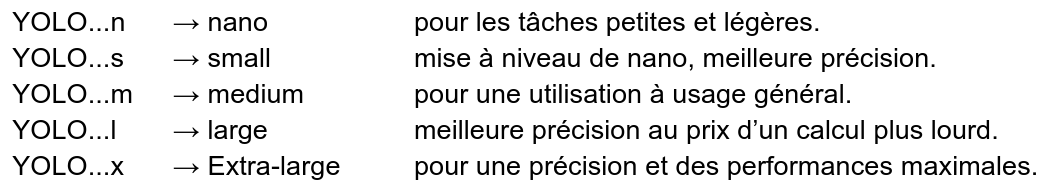
\includegraphics[width=1.\textwidth]{images/YOLO_nsmlx.png}\\}
        \only<3>{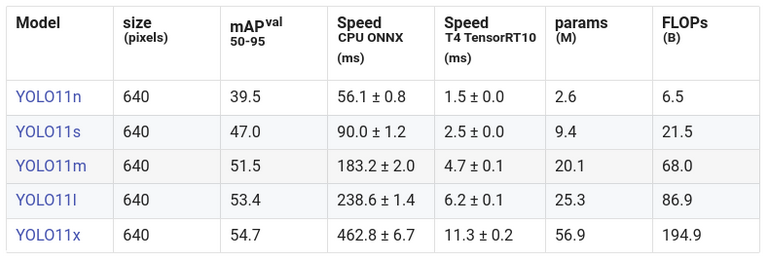
\includegraphics[width=\textwidth]{images/YOLO11_architectures.png}\\}
        \only<4,5>{$\leadsto$ Les versions {\bf n} et {\bf s} sont retenues (cible RPi4)\\}
        \only<5>{$\leadsto$ 4 réseaux utilisés\\
          \fileBF{YOLOv8n}, \fileBF{YOLOv8s}, \fileBF{YOLO11n}, \fileBF{YOLO11s}}
        }
    \end{itemize}
    
  \end{tcolorbox}
    
\end{frame}
%=============================================================

%====== #31 ==================================================
\begin{frame}{Détection d'objets 3D : entraînement du réseau YOLO}
  
  \begin{tcolorbox}[title={Choix des méta-paramètres d’entraînement}]
    Méta-paramètres \Chocolate{batch} et \Chocolate{epochs}

    {\tiny étude v1}\\[1mm]
      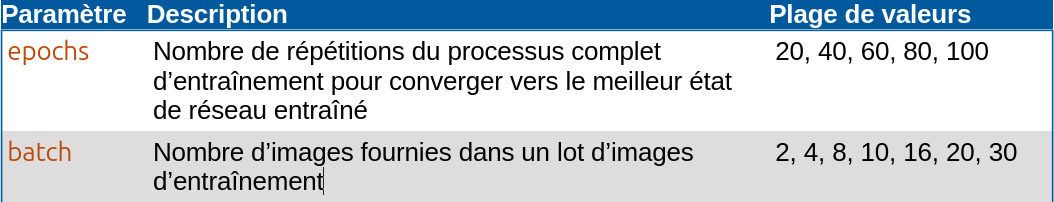
\includegraphics[width=\textwidth]{images/ChoixMetaParamV1.png}

    {\tiny étude v2}\\[1mm]
      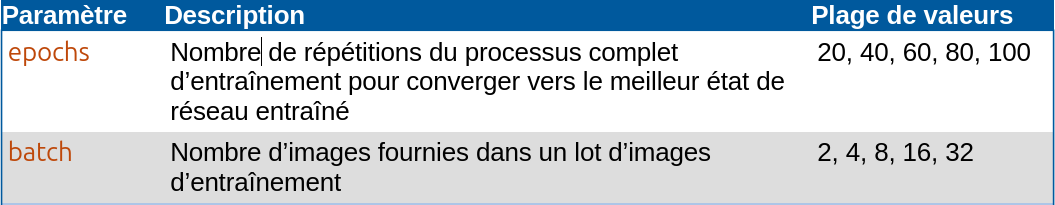
\includegraphics[width=\textwidth]{images/ChoixMetaParamV2.png}

  \end{tcolorbox}
    
\end{frame}
%=============================================================

%====== #32 ==================================================
\begin{frame}{Détection d'objets 3D : entraînement du réseau YOLO}
  
  \begin{tcolorbox}[title={Choix des paramètres d’entraînement}]
    Paramètres \Chocolate{imgz}, \Chocolate{pretrained} et \Chocolate{seed}:\\[5mm]
   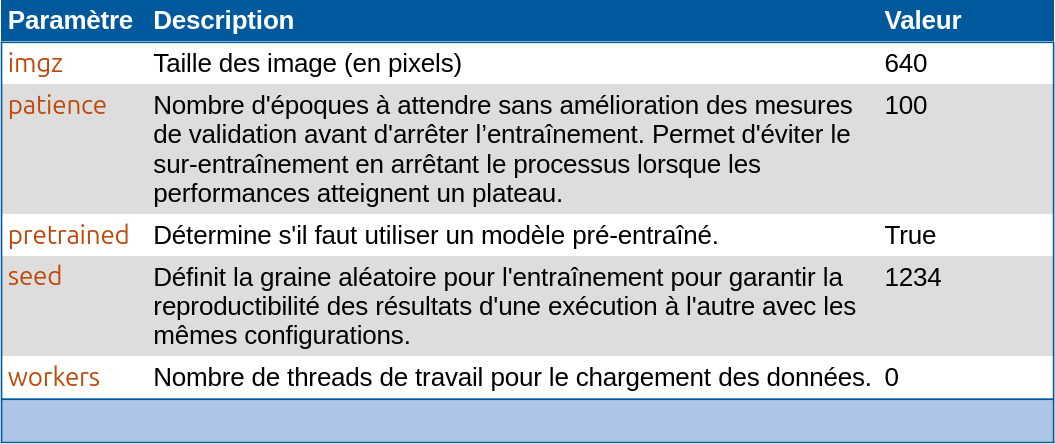
\includegraphics[width=\textwidth]{images/ChoixParam.png}
  \end{tcolorbox}
    
\end{frame}
%=============================================================

%====== #33 ==================================================
\begin{frame}{Détection d'objets 3D : entraînement du réseau YOLO}
  
  {\small La combinaison des méta-paramètres donne de nombreux entraînements à stocker :\\
  4 x 7 x 5 = 140 entraînements pour l'étude V1, 100 pour l'étude V2.}
  
  \only<2->{
    \begin{tcolorbox}[title={Nommage des dossiers d'entraînement (exemple V2)}]
    \includegraphics[width=\textwidth]{images/Regle_nommage.png}

    {\small   
      \bfdarkchoco{vvv} $\leadsto$ version du réseau YOLO : (\Chocolate{v8n}, \Chocolate{v8s}, \Chocolate{11n}, \Chocolate{11s})
              
      \bfdarkchoco{BB} $\leadsto$ méta-paramètre \Chocolate{batch} : 
      (\Chocolate{02}, \Chocolate{04}, \Chocolate{08}, \Chocolate{16}, \Chocolate{32})
              
      \bfdarkchoco{EEE} $\leadsto$ méta-paramètre \Chocolate{epochs} : 
      (\Chocolate{020}, \Chocolate{040}, \Chocolate{060}, \Chocolate{080}, \Chocolate{100})
    }
    \end{tcolorbox}
    }

  \only<3->{
    \begin{tcolorbox}[add to width=.7cm, title={Programmes Python d'entraînement des réseaux YOLO}]
      \fileBF{train\_YOLOv8.py} et  \fileBF{train\_YOLO11.py} développés pour l'étude V1, complétés pour V2.
    \end{tcolorbox}
    }
    
\end{frame}
%=============================================================

%====== #34 ==================================================
\begin{frame}{Détection d'objets 3D : entraînement du réseau YOLO}
  
  Les entraînements sont faits sur un PC équipé d'une carte graphique \textbf{Nvidia Quadro TRX8000}.

  \begin{tcolorbox}[title={Contenu des dossiers d'entraînement\\ \textbf{UCIA-YOLOvvv/batch-BB\_epo-EEE/}}, height=60mm]
    
    \begin{itemize} 
    \item<2-> Extraits des images d'entraînement\\
      \only<3>{\vspace*{-2cm}\hspace*{5.8cm}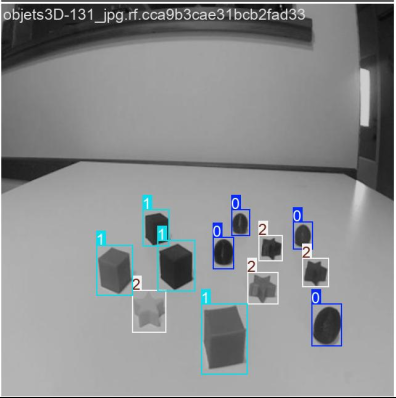
\includegraphics[height=.5\textwidth]{images/Exple_image_train_v2.png}}
    \item<4-> Résultats avec les images de validation  \\
      \only<5>{\vspace*{-2.5cm}\hspace*{5.8cm}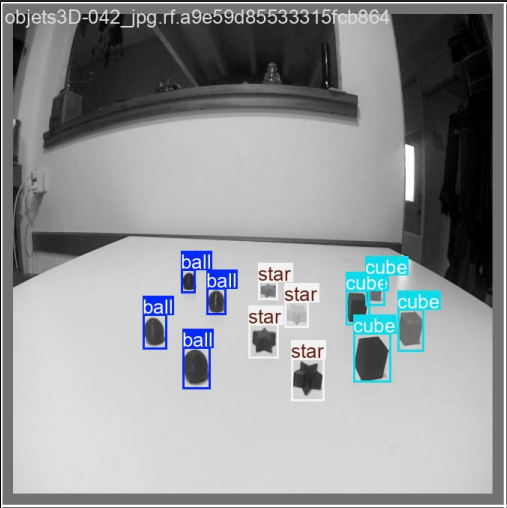
\includegraphics[height=.5\textwidth]{images/Exple_image_val_v2.png}}
    \item<6-> Fichier \fileBF{confusion\_matrix.png} : matrice de confusion \\
      \only<7>{\vspace*{-5.5cm}\hspace*{1.cm}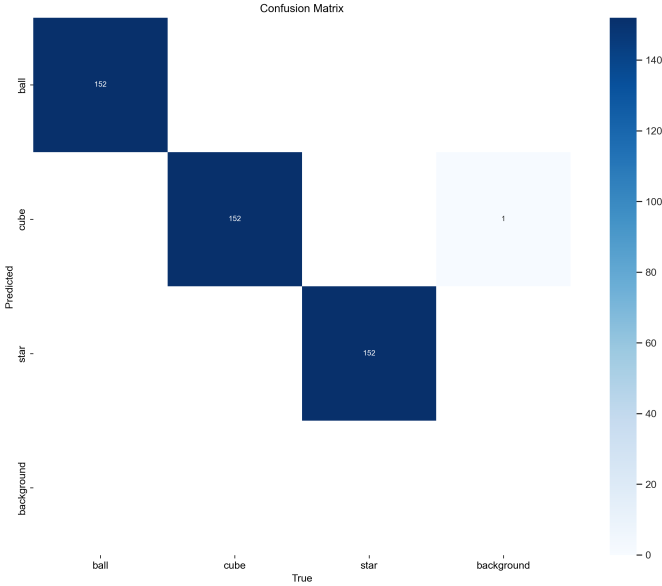
\includegraphics[height=.85\textwidth]{images/ConfusionMatrix_v2.png}}
    \item<8-10> Fichier \fileBF{results.png} : tracé des statistiques et métriques d'entraînement\\
      \only<9>{\vspace*{-4.6cm}\hspace*{-1.8cm}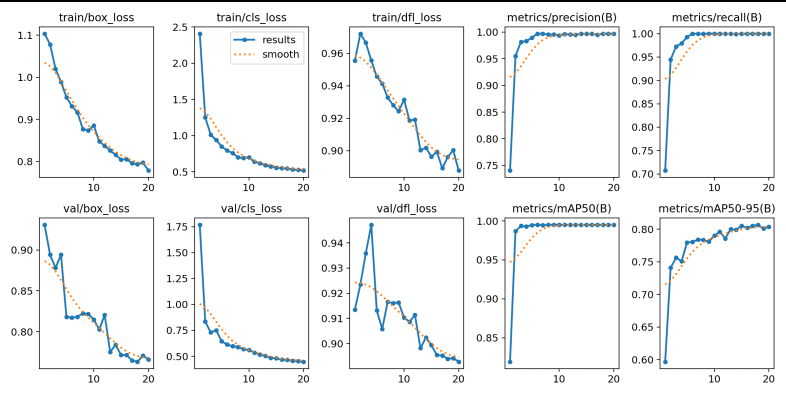
\includegraphics[width=1.3\textwidth]{images/Metrics_v2.png}}
    \end{itemize}
    
  \end{tcolorbox}
    
\end{frame}
%=============================================================

%====== #35 ==================================================
\begin{frame}{Détection d'objets 3D : entraînement du réseau YOLO}
  
  \begin{tcolorbox}[title={Contenu des dossiers des poids\\ \textbf{UCIA-YOLOvvv/batch-BB\_epo-EEE/weights}}, height=68mm]
    \begin{itemize}
    \item<1-> \fileBF{best.pt} : fichier binaire des poids du réseau entraîné \\(au format \Chocolate{pytortch}).\smallskip
    \item<2-> Formats optimisés générés pour RPi4 :
      \visible<2->{
        \begin{itemize}
        \item \fileBF{best.onnx} : poids du réseau entraîné au format \href{https://docs.ultralytics.com/fr/integrations/onnx/}{ONNX}
        \item \fileBF{best.ncmm} : poids du réseau entraîné au format \href{https://docs.ultralytics.com/fr/integrations/ncnn/}{NCNN}
        \end{itemize}
        \smallskip
        }
    \item<3-> Taille des fichiers binaires des poids des réseaux YOLO
      \only<3->{\\[1mm]\hspace*{1cm}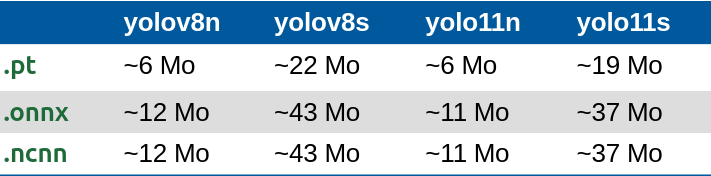
\includegraphics[width=.7\textwidth]{images/Taille_fichiers_poids.png}}
    \end{itemize}
    
  \end{tcolorbox}
    
\end{frame}
%=============================================================

%====== #36 ==================================================
\begin{frame}{Détection d'objets 3D : Performances entraînements}

  \begin{itemize}
  \item Le module Python \textbf{ultralytics} fournit des fonctions pour évaluer les
    indicateurs de performance de détection d'objets.\smallskip
    
  \visible<2->{\item Programmes \fileBF{eval\_YOLOv8.py} et \fileBF{eval\_YOLO11.py} développés 
    (V1 et V2) pour évaluer les différentes versions d’entraînement des réseaux YOLO.\smallskip}
    
  \visible<3->{\item $\leadsto$ 4 fichiers résultats (exemple pour V2): \\
    \fileBF{results\_yolov8n-V2.txt},  \fileBF{results\_yolov8s-V2.txt},
    \fileBF{results\_yolo11n-V2.txt},  \fileBF{results\_yolo11s-V2.txt}, 
    contenant chacun les valeurs des indicateurs de performance pour les différentes valeurs des méta-paramètres.}
    
  \end{itemize}
    
\end{frame}
%=============================================================

%====== #37 ==================================================
\begin{frame}{Détection d'objets 3D : Performances entraînements}
  
  \begin{tcolorbox}[title={Temps moyen d'inférence}]

    Pour info, sur le PC de calcul (carte {\em Nvidia Quadro TRX8000})
    
    \center\includegraphics[width=.5\textwidth]{images/Temps_moyen_Inférences.png}

    $\leadsto$ Architecture \Chocolate{s} deux fois plus lente que \Chocolate{n}
  \end{tcolorbox}
    
\end{frame}
%=============================================================

%====== #38 ==================================================
\begin{frame}{Détection d'objets 3D : Performances entraînements}
 
  \begin{tcolorbox}[title=Indicateurs de précision détection des réseaux détecteur, add to width=.7cm, height=68mm]
    {\small
      \fileBF{process\_results.py} $\leadsto$ synthèse des évaluation des réseaux entraînés.
      \begin{itemize}
      \item<2-> \Chocolate{recall} : capacité du réseau à identifier toutes les objets dans les images.
      \item<3-> \Chocolate{mAP50} : précision moyenne pour un seuil d'{\em intersection sur union}
        \href{https://medium.com/@prathameshamrutkar3/the-complete-guide-to-object-detection-evaluation-metrics-from-iou-to-map-and-more-1a23c0ea3c9d}{IoU} de 0.5 
        (détections "faciles").\\
        \only<4>{\vspace*{-2cm}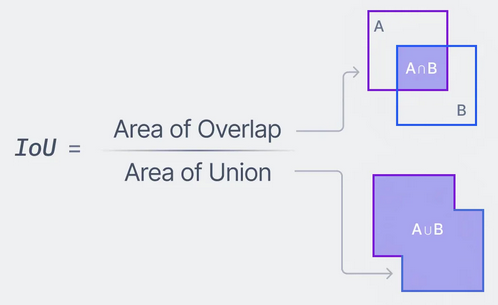
\includegraphics[width=.7\textwidth]{images/IoU-4.png}}
        \only<5>{\vspace*{-2cm}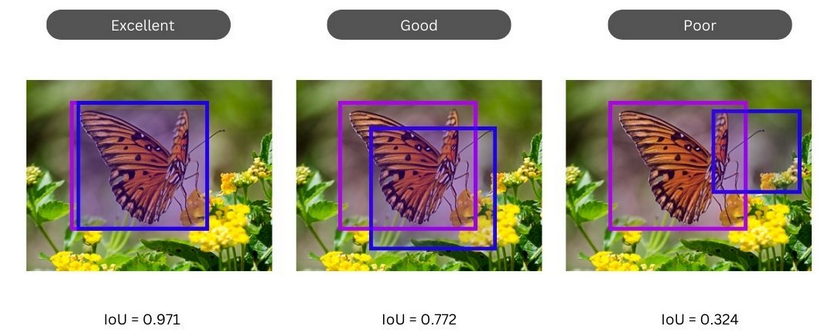
\includegraphics[width=.9\textwidth]{images/IoU-3.png}}
      \item<6-> \Chocolate{mAP50-95} : précision moyenne pour différents seuils \textbf{IoU} allant de 0.5 à 0.95
        (différents niveaux de difficulté de détection).
      \item<7-> \Chocolate{fitness} = 0.1*\Chocolate{mAP50} + 0.9*\Chocolate{mAP50-95}
      \end{itemize}
    }
    \only<8> {\vspace*{-6.8cm}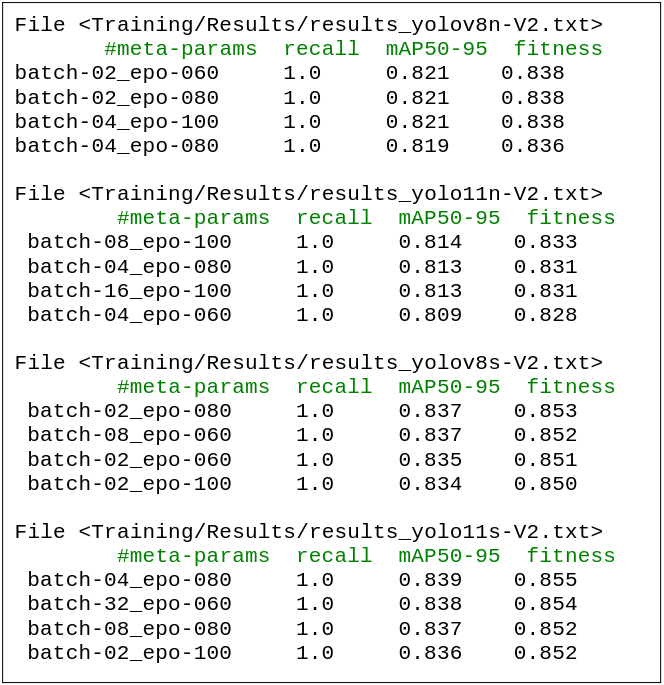
\includegraphics[width=.75\textwidth]{images/Results_recall_mAP50-95_V2.png}}
  \end{tcolorbox}
  
\end{frame}
%=============================================================

%====== #39 ==================================================
\begin{frame}{Détection d'objets 3D : Performances entraînements}
 
  \begin{tcolorbox}[title={Configurations d'entraînement à tester sur RPi4}]
    
    Meilleures performance :

      \begin{itemize}
      \item \fileBF{UCIA-YOLOv8n/batch-04\_epo-100} 
      \item \fileBF{UCIA-YOLOv8s/batch-02\_epo-080}
      \item \fileBF{UCIA-YOLO11n/batch-02\_epo-100}
      \item \fileBF{UCIA-YOLO11s/batch-04\_epo-080} 
      \end{itemize}

      \medskip
      \visible<2>{
      On retrouve des tendances connues :
      \begin{itemize}
      \item \Chocolate{batch\_size} petit $\leadsto$ favorise en entraînement de qualité, 
      \item \Chocolate{epochs} elévé $\leadsto$ compense le petit nombre d'images fournies à chaque entraînement.
      \end{itemize}
      }
  \end{tcolorbox}
    
\end{frame}
%=============================================================

\section{Mise en oeuvre RPi4}

\subsection{Configuration RPi4-UCIA}

%====== #40 ==================================================
\begin{frame}{}

  \vfill
  \center{\Large Étude : Exploitation sur RPi4 des réseaux entraînés YOLO selon le CDC UCIA\\[5mm]
    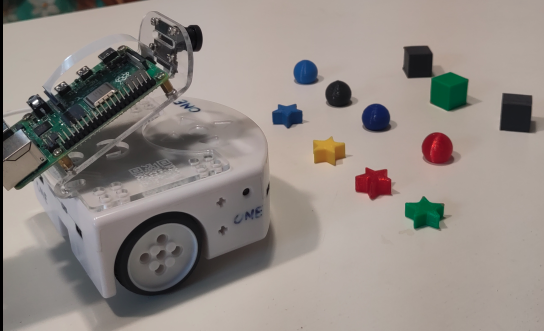
\includegraphics[width=.6\textwidth]{images/V2-Camera-Thymio.png}
    }
  \vfill

\end{frame}
%=============================================================

%====== #41 ==================================================
\begin{frame}{Configuration RPi4-UCIA}
  
  \begin{tcolorbox}[title={Configuration RPi4-UCIA}, height=68mm]
     \begin{itemize}
      \item<1-> Carte micro-SD rapide de 64 GB
      \item<2-> Flash carte micro-SD :\\système d'exploitation \textbf{Rapberry PI OS (64-bit)}\\
        \only<3>{\vspace*{-3cm}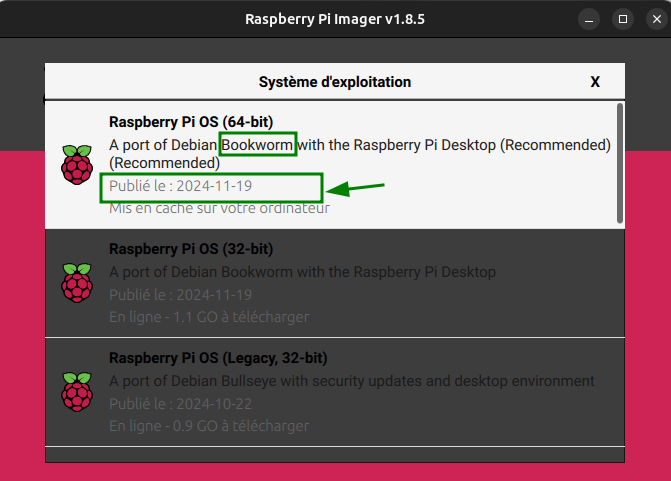
\includegraphics[height=.6\textwidth]{images/PiImager.png}}
      \item<4-> Point d'accès Wifi [SSID : \Chocolate{RPi4-UCIA}, clef :\Chocolate{poppy!station}]\\
        \only<5>{\vspace*{-3cm}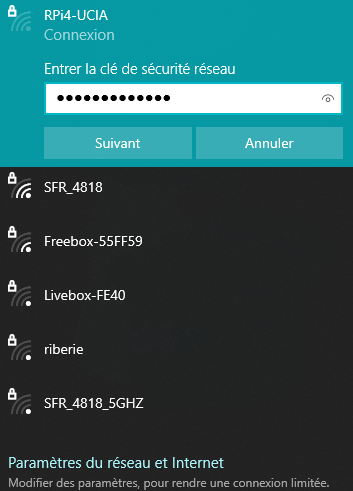
\includegraphics[height=.7\textwidth]{images/Ws_WiFi_suivant-2.png}}
      \item<6-> Compte : \comBF{ucia}, mdp : \comBF{poppy!station}\\
        ouvert automatiquement au démarrage de la RPi4
      \item<7-> Environnement Virtuel Python (EVP) \comBF{vision}\\
        activé automatiquement à l'ouverture du compte \comBF{ucia}
      \item<8-> Arborescence des réseaux YOLO entraînés copiée sur la carte micro-SD.\\
        \only<9>{\vspace*{-7cm}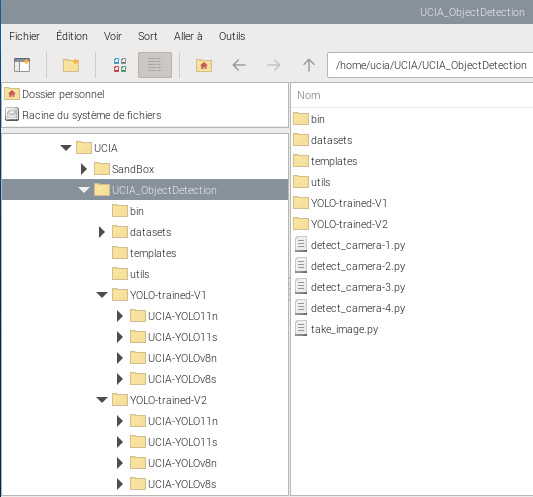
\includegraphics[height=.8\textwidth]{images/RPi4-UCIA_YOLOs-tree.png}}
      \end{itemize}
    
  \end{tcolorbox}
    
\end{frame}
%=============================================================

%====== #42 ==================================================
\begin{frame}{Configuration RPi4-UCIA}
  
  \begin{tcolorbox}[title={Programmes Python d'exploitation des réseaux YOLO}, add to width=.7cm, height=68mm]
    {\small
      \begin{itemize}
      \item<1-> 4 programmes Python \fileBF{detect\_camera-n.py} (n=1,2,3,4) :
      \item<2-> \fileBF{detect\_camera-1.py} : images (N\&B) des détections du réseau YOLO choisi 
        + infos élémentaires sur les détections\\
        \only<3> {\vspace*{-3.5cm}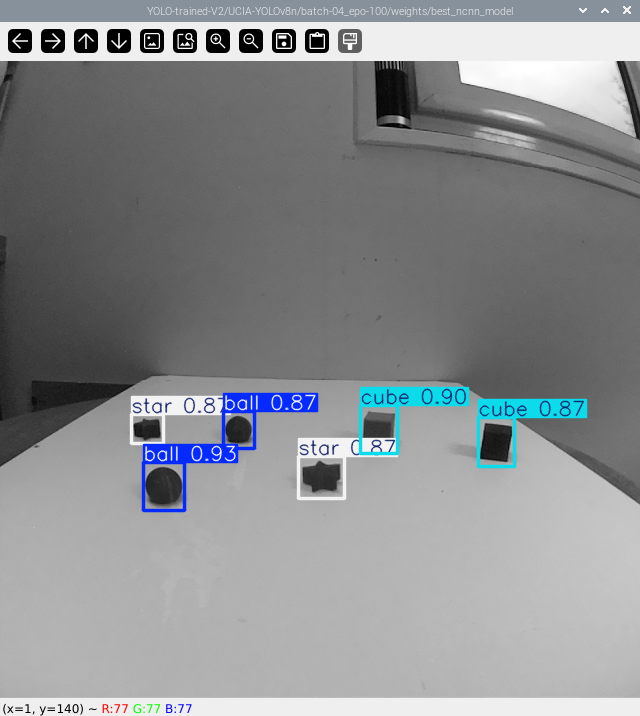
\includegraphics[width=.7\textwidth]{images/detect_camera-1_a.png}}
        \only<4> {\vspace*{-3.5cm}\hspace*{-15mm}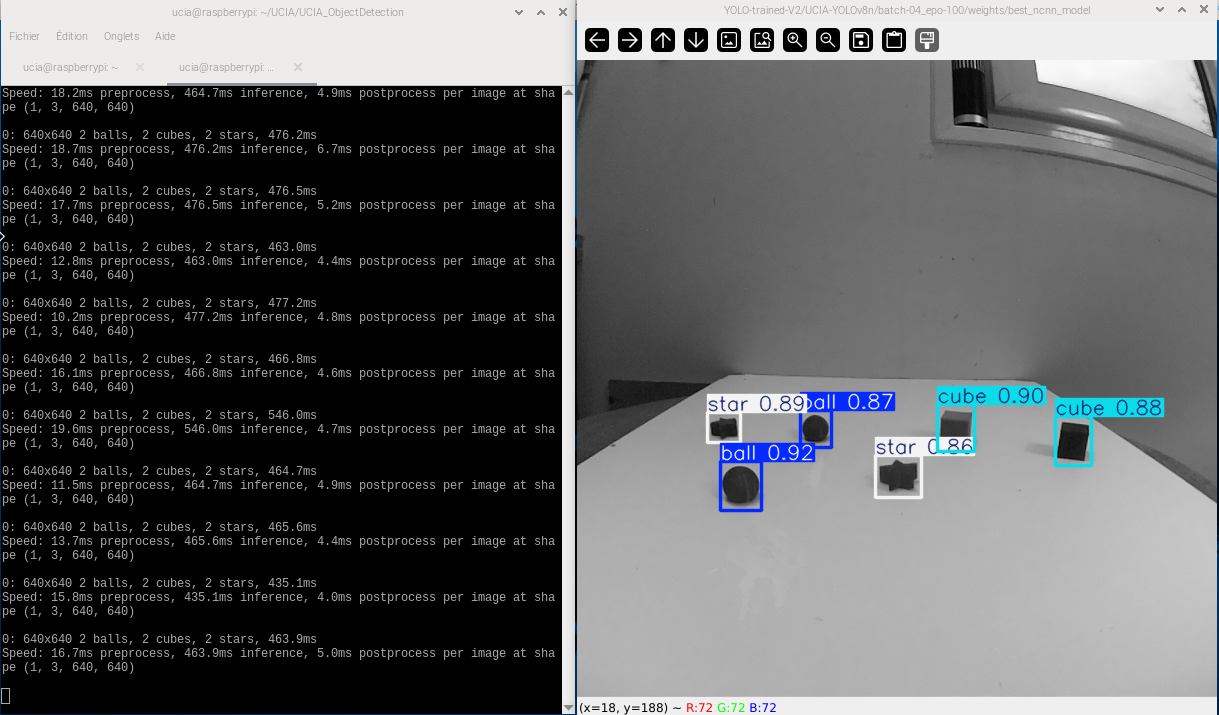
\includegraphics[width=1.2\textwidth]{images/detect_camera-1_b.png}}
      \item<5-> \fileBF{detect\_camera-2.py} : images (couleur) des détections du réseau YOLO choisi 
        + infos détaillées sur les détections\\
        \only<6> {\vspace*{-4cm}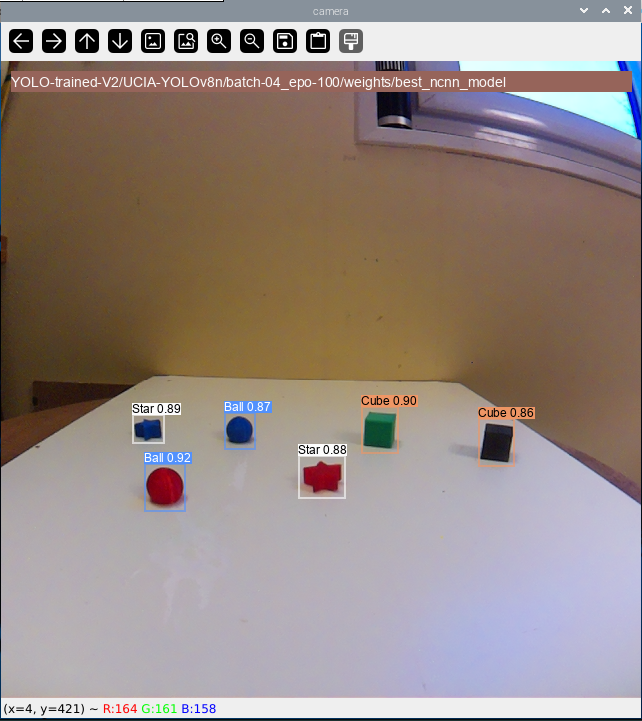
\includegraphics[width=.7\textwidth]{images/detect_camera-2_a.png}}
        \only<7> {\vspace*{-4cm}\hspace*{-15mm}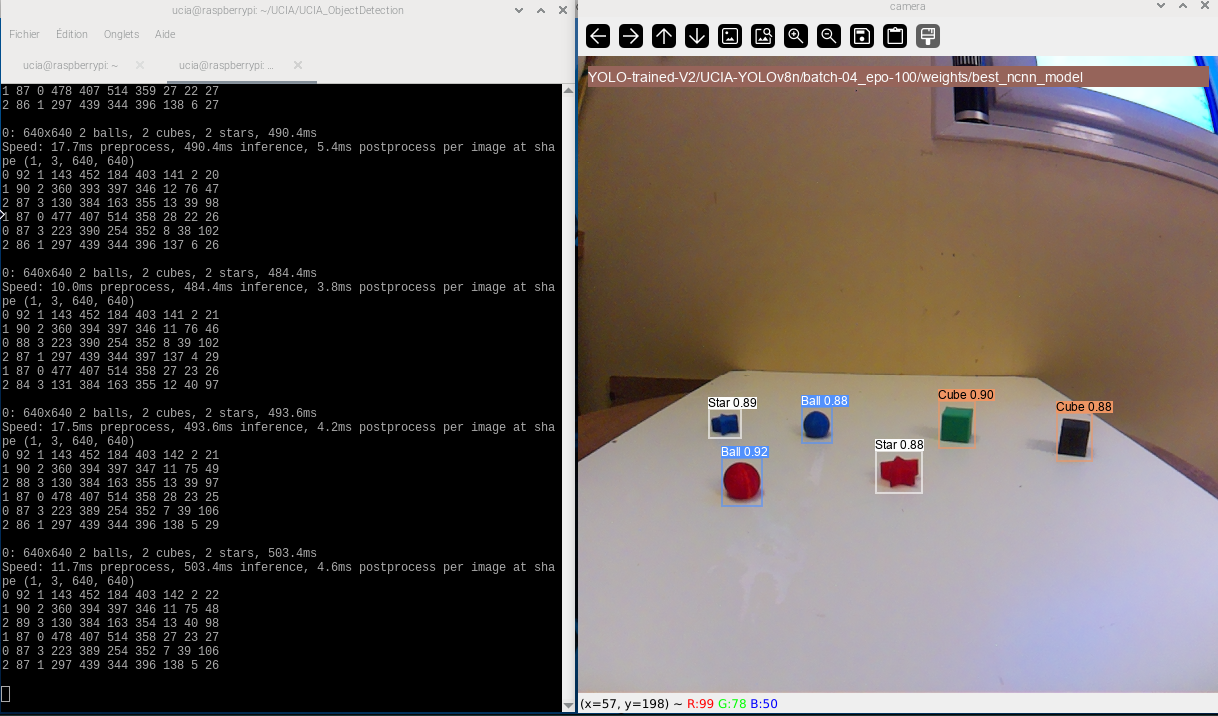
\includegraphics[width=1.2\textwidth]{images/detect_camera-2_b.png}}
      \item<8-> \fileBF{detect\_camera-3.py} : serveur à l'adresse \Chocolate{10.99.99.1:5000/video}\\
        en attente de la connexion d'un navigateur WEB sur cette URL.
        \begin{itemize}
        \item Connexion sur \Chocolate{10.99.99.1:5000/quit} $\leadsto$ terminer l'application\\
        \item Connexion sur \Chocolate{10.99.99.1:5000/halt} $\leadsto$ Shutdown de la carte RPi4 (permet l'extinction)
        \end{itemize}
        \only<9>  {\vspace*{-6cm}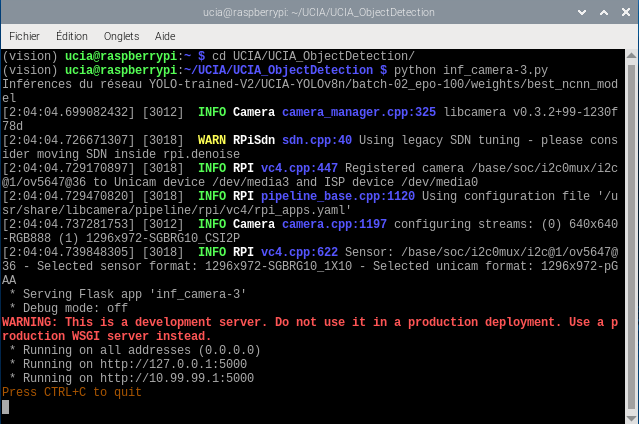
\includegraphics[width=.9\textwidth]{images/detect_camera-3_a.png}}
        \only<10> {\vspace*{-7.5cm}\includegraphics[width=.65\textwidth]{images/detect_camera-3_b.png}}
        \only<11> {\vspace*{-6cm}\includegraphics[width=.9\textwidth]{images/detect_camera-3_c.png}}
      \item<13> Temps d'inférence du réseau \fileBF{YOLOv8n} < ~0.5 seconde
      \end{itemize}
    }
    
  \end{tcolorbox}
    
\end{frame}
%=============================================================

%====== #43 ==================================================
\begin{frame}{Configuration RPi4-UCIA}
  
  \begin{tcolorbox}[title=Exploitation des réseaux YOLO : Bureau à distance (VNC), add to width=.7cm, height=68mm]
    {\small
      \begin{itemize}
      \item<1-> Démarrage RPi4 $\leadsto$ lancement de \fileBF{detect\_camera-3.py}\\
        en attente de l'ouverture de \Chocolate{10.99.99.1:5000/video} par un navigateur... 
        \Chocolate{CTRL + C} pour quitter et fermer le terminal.
      \item<2-> Double clic icone [Ai] $\leadsto$ lancement de \fileBF{detect\_camera-3.py} : \\
        en attente de l'ouverture de \Chocolate{10.99.99.1:5000/video} par un navigateur... 
        \Chocolate{CTRL + C} pour quitter et fermer le terminal.\\
        \only<3>  {\vspace*{-2.5cm}\includegraphics[width=.9\textwidth]{images/Bureau-distance-iconeAI.png}}
      \item<4-> Connexion sur \Chocolate{10.99.99.1:5000/quit} $\leadsto$ terminer l'application\\
      \item<4-> Connexion sur \Chocolate{10.99.99.1:5000/halt} $\leadsto$ Shutdown de la carte RPi4 (permet l'extinction)
      \end{itemize}
    }
  \end{tcolorbox}
    
\end{frame}
%=============================================================

%====== #44 ==================================================
\begin{frame}{Configuration RPi4-UCIA}
  
  \begin{tcolorbox}[title=Exploitation des réseaux YOLO : Navigateur web, add to width=.7cm, height=68mm]
    {\small
      \begin{itemize}
      \item<1-> Démarrage RPi4 $\leadsto$ lancement de \fileBF{detect\_camera-3.py}\\
        en attente sur \Chocolate{10.99.99.1:5000/video} par un navigateur... 
      \item<2-> Connexion navigateur sur \Chocolate{10.99.99.1:5000/video}\\
        $\leadsto$ images (couleur) des détections du réseau YOLO\\
        \only<3> {\vspace*{-3cm}\includegraphics[width=.65\textwidth]{images/detect_camera-3_b.png}}
      \item<4-> Connexion navigateur sur \Chocolate{10.99.99.1:5000/quit}\\
        $\leadsto$ terminer l'application
      \item<4-> Connexion navigateur sur \Chocolate{10.99.99.1:5000/halt}\\
        $\leadsto$ Shutdown de la carte RPi4 (permet l'extinction)
      \end{itemize}
    }
    
  \end{tcolorbox}
    
\end{frame}
%=============================================================

%====== #45 ==================================================
\begin{frame}{Configuration RPi4-UCIA}
  
  \begin{tcolorbox}[title=Exploitation des réseaux YOLO : Navigateur web, add to width=.7cm, height=68mm]
    {\small
      \begin{itemize}
      \item<2-> Connexion sur \Chocolate{10.99.99.1:5000/video} $\leadsto$ images (couleur) des détections du réseau YOLO\\
        \only<3> {\vspace*{-3cm}\includegraphics[width=.6\textwidth]{images/detect_camera-3_b.png}}
      \item<4-> Connexion sur \Chocolate{10.99.99.1:5000/quit} $\leadsto$ terminer l'application
      \item<4-> Connexion sur \Chocolate{10.99.99.1:5000/halt} $\leadsto$ Shutdown de la carte RPi4 (permet l'extinction)
      \end{itemize}
    }
    
  \end{tcolorbox}
    
\end{frame}
%=============================================================

\subsection{Formats de réseau entraîné optimisé pour RPi4}

\subsection{Point d'accès WiFi}

\subsection{}

\subsection{}


\section{References}

%=============================================================
\begin{frame}{References}
  
  \noindent\fontsize{8}{8}\selectfont{

    \begin{itemize}
      \item UCIA Cahier des charges : Robot ROSA avec Intelligence Artificielle OpenSource et OpenHardware \smallskip

      \item Page du site roboflow pour l’accès publique au jeu de données de l’étude :\\
        \href{https://universe.roboflow.com/ucia/ucia-ia-object-detection/dataset/2}
             {https://universe.roboflow.com/ucia/ucia-ia-object-detection/dataset/2} \smallskip

      \item «Ultralytics YOLO11: Faster Than You Can Imagine!», Ankan Ghosh, October 8, 2024\\
        \href{https://learnopencv.com/yolo11/}{https://learnopencv.com/yolo11/} \smallskip
         
      \item Article WikiPédia sur les indicateurs de précision:\\
        \href{https://fr.wikipedia.org/wiki/Pr\%C3\%A9cision\_et\_rappel}
             {https://fr.wikipedia.org/wiki/Pr\%C3\%A9cision\_et\_rappel} \smallskip

      \item «Analyse approfondie des mesures de performance», site Ultralytics\\
        \href{https://docs.ultralytics.com/fr/guides/yolo-performance-metrics/}
             {https://docs.ultralytics.com/fr/guides/yolo-performance-metrics/} \smallskip

      \item «The Complete Guide to Object Detection Evaluation Metrics: From IoU to mAP and More»\\
        \href{https://medium.com/@prathameshamrutkar3/the-complete-guide-to-object-detection-evaluation-metrics-from-iou-to-map-and-more-1a23c0ea3c9d}
             {https://medium.com/@prathameshamrutkar3/the-complete-guide-to-object-detection-evaluation-metrics-from-iou-to-map-and-more-1a23c0ea3c9d}

    \end{itemize}
  }
  
\end{frame}

%=============================================================

\section{Annexes}

%====== #43 ==================================================
\begin{frame}{}

  \vfill
\center{Annexes techniques}
  \vfill

\end{frame}
%=============================================================

\subsection{Supervised learning}

%====== #44 ==================================================
\begin{frame}{}

  {\small
    \vspace*{-1mm}\hspace*{-10mm}\includegraphics[width=1.18\textwidth]{./images/NetworkTraining.png}
  \vspace*{-4mm}\begin{itemize}
  \item The dataset is split into (mini) {\bf batches} of size \code{batch\_size}
  \item After each {\em feed forward} the {\em Back Propagation} algorithm modifies the weights
    neurons to minimize the error $e$.
  \end{itemize}
  }
\end{frame}
%=============================================================

%====== #45 ==================================================
\begin{frame}{}
  \includegraphics[width=\textwidth]{./images/NetworkTraining_2.png}
  {\small
    \vspace*{-5mm}\begin{itemize}
    \item Training with the whole dataset is repeated \code{n\_epoch} times,
    \item The network state at the end of epoch \code{n} becomes the initial state for epoch \code{n+1}.
    \end{itemize}
    }
\end{frame}
%=============================================================

\end{document}


      \item<12-> \fileBF{detect\_camera-3.py} : lancement du serveur web à l'adresse \Chocolate{http://10.99.99.1:5000/video}...\\
        en attente de la connexion d'un navigateur WEB sur cette URL et du lancement du programme de pilotage Thymio.\\
        \only<9> {\vspace*{-5cm}\includegraphics[width=.9\textwidth]{images/detect_camera-3_a.png}}
        \only<10> {\vspace*{-6.5cm}\includegraphics[width=.7\textwidth]{images/detect_camera-3_b.png}}
        \only<11> {\vspace*{-5cm}\includegraphics[width=.9\textwidth]{images/detect_camera-3_c.png}}



        
[ML-01] – JLC  
« Machine Learning for Humans » 
https://medium.com/machine-learning-for-humans

Point d'entrée du site « Machine Learning for Humans », à partir duquel on peut aller sur "A Beginner's Guide to AI/ML" et d'autres documents très intéressants.


[ML-02] – JLC  
« A Beginner’s Guide to AI/ML »
https://medium.com/machine-learning-for-humans/why-machine-learning-matters-6164faf1df12

Cours complet : supervised learning, unsupervised learning, Neural networks & deep learning, reinforcement learning....Version PDF du cours également disponible. sur : https://www.dropbox.com/s/e38nil1dnl7481q/machine_learning.pdf?dl=0

[ML-03] – VG
« ML Basics : Unsupervised, supervised and reinforcement learning »
Article court mais utile pour bien saisir la différence entre supervised, unsupervised et reinforcement learning.
https://medium.com/@machadogj/ml-basics-supervised-unsupervised-and-reinforcement-learning-b18108487c5a

DRL  (Deep Reinforcement Learning)
[DRL-01] – JLC 
« Introduction to Various Reinforcement Learning Algorithms. Part I (Q-Learning, SARSA, DQN, DDPG) »
https://towardsdatascience.com/introduction-to-various-reinforcement-learning-algorithms-i-q-learning-sarsa-dqn-ddpg-72a5e0cb6287

[DRL-02] – VG
https://deepmind.com/blog/deep-reinforcement-learning/
Récapitulatif de ce qu’on sait faire aujourd’hui en DRL fait par DeepMind (un des leaders mondiaux en DRL, concepteurs d’AlphaGo notamment) 

[DRL-03] – JLC
« Demystifying Deeep Reinforcement Learning », Tambet Matiisen
https://neuro.cs.ut.ee/demystifying-deep-reinforcement-learning/
Article très clair et très pédagogique sur ML, RL et DQN.

\footnote{\tiny \hyperlink{DeepLeraning}{[2]} {\em Deep Learning.}, Goodfellow {\em et al.}, Chapitre {\em "6.5 Back-Propagation and Other Differentiation Algorithms"}}

IBM Watson https://www.ibm.com/watson/products-services

*******************
*******************

    one episode = one a sequence of states, actions and rewards, which ends with terminal state. For example, playing an entire game can be considered as one episode, the terminal state being reached when one player loses/wins/draws. Sometime, one may prefer to define one episode as several games (example: "each episode is a few dozen games, because the games go up to score of 21 for either player").
    one epoch = one forward pass and one backward pass of all the training examples, in the neural network terminology.

    \subsection{Neural Networks achitectures}

%=============================================================
\begin{frame}{Neural Network Architectures}

  Examples of common NN architectures:
\begin{itemize}
  \item \bfdarkchoco{Dense} Sequential (DNN): the simplest NN made of successive layers of neurones, with {\em Feed Forward} and {\em Back Propagation} algorithms.
  \item \bfdarkchoco{Convolutional} (CNN): Mostly used for analyzing and classifying images.
  \item \bfdarkchoco{Recurrent} (RNN): Used to learn from time series, like the Long short-term memory (LSTM) algorithm.
  \item \bfdarkchoco{Generative adversarial} (GAN): can generate images, text...
\end{itemize}
\end{frame}
%=============================================================

%=============================================================
\begin{frame}
  \begin{tcolorbox}[title={RL ingredients: \textbf{Policy}, \textbf{Value function}}, fonttitle=\Large]    
    \begin{itemize}
    \item <1-> The \bfdarkchoco{Policy} $\pi(a|s)$ is a probalistic mapping between action $a$ and state $s$.
      \begin{itemize}
      \item <2-> can be as simple as a look-up table (Q-learning) or involve extensive computation.
      \end{itemize}
      \item Is the core of a DRL in the sense that it alone is sufficient to determine behavior.
    \item <3-> The \bfdarkchoco{Value function} selects actions that bring states of the highest value over the long run.
    \end{itemize}    
  \end{tcolorbox}
\end{frame}
%=============================================================

\subsection{Activation functions SoftMax}

%====== #46 ==================================================
\begin{frame}{Computing aspects}
  \vspace*{-2mm}

  \begin{itemize}
    
  \item intermediate layers $\leadsto$ \bfdarkchoco{relu} promotes network learning
    \footnote{{\tiny avoids the {\em vanishing gradient} that appears in {\em back propagation}}}.\smallskip
    
  \item \bfdarkchoco{softmax} always used for in the last layer for {\bf Classifying}.
    
  \end{itemize}
  \smallskip
  
  \begin{tcolorbox}[add to width=.7cm, title={Example: ativation function {\em softmax} for the last layer, 10 classes}]
    
    \begin{minipage}{.55\textwidth}
      \vspace*{-2mm}\includegraphics[width=0.8\textwidth]{images/softmax-2.png}
    \end{minipage}\hspace*{5mm}\begin{minipage}{.45\textwidth}
      {\small
        \begin{itemize}
        \item The activation of neuron $k$ is $Y_k = e^{y_k}/\sum_i{e^{y_i}}$
          with $y_k = \sum_i \omega_i x_i - b$ calculated by the neuron $k$.
        \item The neurons outputs are interpreted as {\bf probabilities} in the interval [0,1].
        \item[\Black{$\leadsto$}] <2> the label of the neuron with the highest probability is the network response
      \end{itemize}}
    \end{minipage}
  \end{tcolorbox}
    
\end{frame}
%=============================================================

\subsection{One-hot coding}

%====== #47 ==================================================
\begin{frame}{Computing aspects [Classification]}

\begin{tcolorbox}[title={\em One-hot} coding of labels]

     Goal: transform the image labels to match the network output (vector of probabiliies):

     {\small
       \begin{itemize}
       \item Image labels: ordered set \textbf{integers}.
       \item Network output: \textbf{vector of \texttt{float}} in the interval [0;1] calculated by the {\em softmax} activation of the output neurons.
       \item {\em One-hot} coding of an ordered set $\mathfrak{L}$ of $N$ labels: \\[1mm]
         - each label value is coded as a vector with $N$ components all zero except one (equal to $1$),\\
         - the rank of the $1$ in the vector gives the value of the labe.
       \end{itemize}
     }
\end{tcolorbox}

\visible<2>{
  \begin{minipage}{.3\textwidth}
    \vspace*{-22mm}\hspace*{-5mm}\includegraphics[width=1.1\textwidth]{images/oneHotCoded.png}
  \end{minipage}
  \begin{minipage}{.6\textwidth}
    \vspace*{-5mm}{\small The {\em one-hot} encoding of the labels '0' to '9' gives a vector with 10 components.}
  \end{minipage}
}
    
\end{frame}
%=============================================================

%====== #48 ==================================================
\begin{frame}{Computing aspects [Classification]}

\begin{tcolorbox}[title=Error function: {\em Cross entropy error}]

  \begin{itemize}
  \item The image analysed by the network $\leadsto$ vector $\hat{Y}$ of \texttt{float} to be compared to the vector $Y$ of the {\em hot-one} encoding of the true image label.
  \item The error (loss) function {\em cross entropy} is adapted to {\em one-hot} coding: $e(Y,\hat{Y})=-\sum_i Y_i\ log(\hat {Y}_i)$\\
    \includegraphics[width=.9\textwidth]{images/CrossEntropyError.png}
  \end{itemize}
  
   \end{tcolorbox}  
\end{frame}
%=============================================================

\subsection{Optimisation}

%====== #49 ==================================================
\begin{frame}{Computing aspects}

\begin{tcolorbox}[title=Optimization and {\em Back Propagation}]

  \begin{itemize}
    \visible<1->{\item During the training an optimization algorithm computes the gradient of the error function
      with respect to the network weights.}
    \visible<2->{\item The {\em Back Propagation} algorithm \textbf{modifies} the weights of the network layer by layer thanks to the gradient of the error function,
      iterating from the last layer to the first layer. }
    \visible<3->{\item Examples of optimization algorithms:
      \begin{itemize}
      \item Gradient Descent ({\em Gradient Descent (GD)})
      \item Stochastic Gradient Descent ({\em Stochastic Gradient Descent (SGD)})
      \item {\em \href{https://arxiv.org/abs/1412.6980}{Adam}} (improved version of gradient descent)...
      \end{itemize}

      {\small The module \href{https://www.tensorflow.org/api_docs/python/tf/keras/optimizers}{tf.keras.optimizers}
        provides Python implementation of several optimization algorithms.}}
      
  \end{itemize}
\end{tcolorbox}

\end{frame}
%=============================================================

\subsection{Back-propgation algorithm}

%====== #50 ==================================================
\begin{frame}{Computing aspects}

  {\small Visualization of iterations of gradient descent algorithms for an very-simple loss function with only 2 variables:}\\[2mm]
  \hspace*{25mm}\href{https://github.com/Jaewan-Yun/optimizer-visualization/blob/master/figures/movie9.gif}{\includegraphics[width=.45\textwidth]{images/adam_plot3D_animated.png}}\\[-2mm]
  %\hspace*{8mm}\includegraphics[width=.8\textwidth]{images/adam_plot3D_animated.png}\\[-2mm]
  %\animategraphics[width=.8\textwidth,controls]{10}{./images/Adam-plot3D/movie9/img_}{0}{114}
  \hspace*{25mm}{\tiny (source: \href{https://github.com/Jaewan-Yun/optimizer-visualization}{github.com/Jaewan-Yun/optimizer-visualization})}
  
  \medskip
      {\small Video explaining the {\em back propagation} algorithm:}\\
      \hspace*{30mm}\href{https://www.3blue1brown.com/lessons/backpropagation}{\includegraphics[width=.35\textwidth]{images/video-BackPropagation.png}}
\end{frame}
%=============================================================
